\begin{savequote}[75mm]
Mathematics is the queen of science
\qauthor{--- Carl Friedrich Gauss ---}
\end{savequote}

\chapter{Vector--valued functions}
\label{chap_vector_fun}
\graphicspath{{figures/Vector_Fun/}}

In Chapter~\ref{chap_vector}, we learned about vectors and we were introduced to the power of vectors within mathematics. In this chapter, we will build on this foundation to define functions whose input is a real number and whose output is a vector. 

\section{Vector--valued functions}\label{sec:vvf}
\subsection{Definition}

We are very familiar with real--valued functions, that is, functions whose output is a real number. This section introduces vector--valued functions -- functions whose output is a vector. 

\ifcalculus
\begin{definition}[Vector--valued function]\label{def:vvf} 
A \textbf{vector--valued function} (\textit{vectorfunctie}) is a function of the form 
$$\vec r(t) = \left(f(t),g(t)\,\right) \quad \text{or}\quad \vec r(t) = \left( \,f(t),g(t),h(t)\,\right),$$
where $f$, $g$ and $h$ are real--valued functions, and are called the \textbf{component functions}.\\

The domain of $\vec r$ is the set of all values of $t$ for which $\vec r(t)$ is defined. The range of $\vec r$ is the set of all possible output vectors $\vec r(t)$.
\index{vector--valued function}\index{function!vector--valued}\index[aut]{vector functie}\index[aut]{functie ! vector}
\end{definition}
\fi

\ifanalysis

\begin{definition}[Vector--valued functions]\label{def:vvf}
A $n$-dimensional \textbf{vector--valued function} (\textit{vectorfunctie}) is a function of the form 
$$\vec r(t) = \left( f_1(t),f_2(t),\ldots,f_n(t)\,\right),$$
where  the $f_i$ are real-valued functions, and are called the \textbf{component functions}.\\

The domain of $\vec r$ is the set of all values of $t$ for which $\vec r(t)$ is defined. The range of $\vec r$ is the set of all possible output vectors $\vec r(t)$.
\index{vector--valued function}\index{function!vector--valued}\index[aut]{vector functie}\index[aut]{functie ! vector}\index[aut]{domein}\index{domain}\index{range}
\end{definition}

\fi

Evaluating a vector--valued function at a specific value of $t$ is straightforward; simply evaluate each component function at that value of $t$. For instance, if $\vec r(t) = \left( t^2,t^2+t-1\right)$, then $\vec r(-2) = \left( 4,1\right)$. We can sketch this vector, as is done in Figure \ref{fig_vector_fun_1a}. Plotting lots of vectors is cumbersome, though, so generally we do not sketch the whole vector but just the terminal point. The graph of a vector--valued function is the set of all terminal points of $\vec r(t)$, where the initial point of each vector is always the origin. In Figure \ref{fig_vector_fun_1b} we sketch the graph of $\vec r$\,; we can indicate individual points on the graph with their respective vector, as shown.

\begin{figure}[H]
\centering
%\right)isebox{0.5cm}{
\centerline{
\subfigure[\label{fig_vector_fun_1a}]{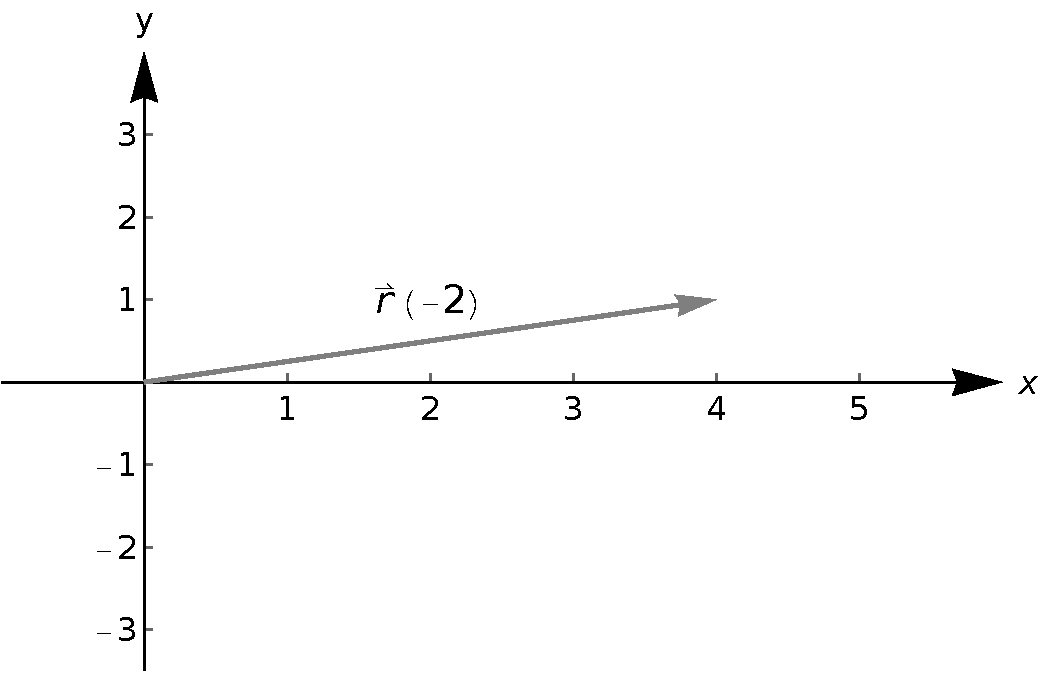
\includegraphics[width=0.43\textwidth]{fig_vector_fun_1a}}
\hspace{0.1cm}
\subfigure[\label{fig_vector_fun_1b}]{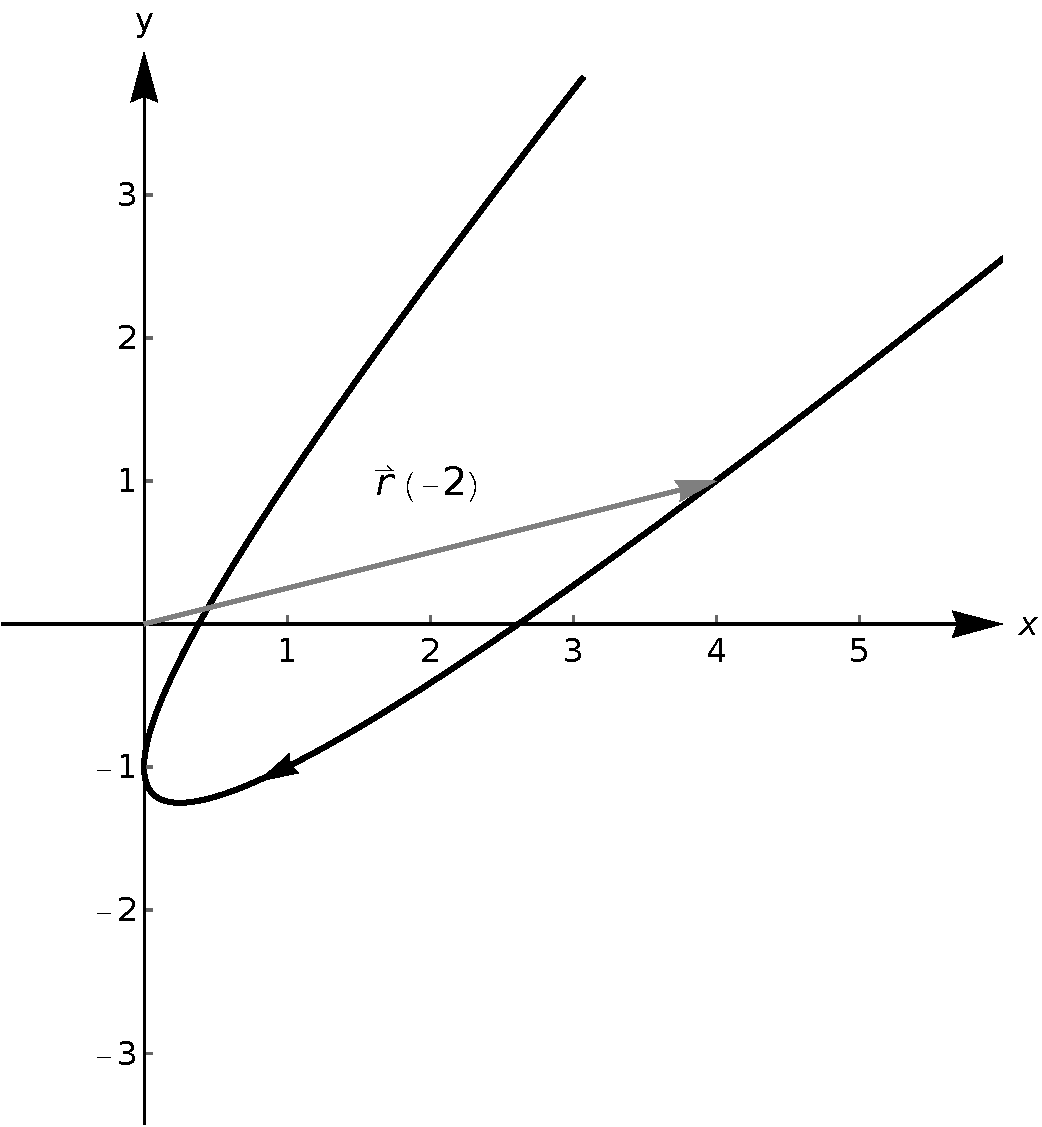
\includegraphics[width=0.35\textwidth]{fig_vector_fun_1b}}
}
\caption{Sketching the graph of a vector--valued function. }
\end{figure}

Vector--valued functions are closely related to parametric equations of graphs. While in both methods we plot points $\big(x(t), y(t)\big)$ or $\big(x(t),y(t),z(t)\big)$ to produce a graph, in the context of vector--valued functions each such point represents a vector. The implications of this will be more fully realized in the next section as we apply calculus ideas to these functions.

\begin{example}\label{ex_vvf2}
Graph $\vec r(t) = \left( \cos (t),\sin (t),t\right)$ for $0\leq t\leq 4\pi$.

\xhrulefill{gray}{2.5pt}Solution \xhrulefill{gray}{2.5pt}

We can plot points, but careful consideration of this function is very revealing. Momentarily ignoring the third component, we see that the $x$- and $y$- components trace out a circle of radius 1 centred at the origin. Noticing that the $z$ component is $t$, we see that as the graph winds around the $z$-axis, it is also increasing at a constant rate in the positive $z$ direction, forming a spiral. This is graphed in Figure \ref{fig_vector_fun_2}. In the graph, $\vec r(7\pi/4)\approx (0.707,-0.707,5.498) $ is highlighted to help us understand the graph.




\end{example}

\begin{figure}
	\begin{center}
			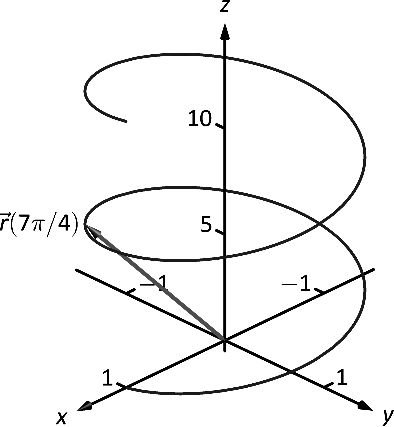
\includegraphics[width=0.4\textwidth]{fig_vector_fun_2}
	\caption{The graph of $\vec r(t)$ in Example \ref{ex_vvf2}.}
	\label{fig_vector_fun_2}
	\end{center}
\end{figure}

\subsection{Algebra of vector--valued functions}\label{subsec:alg_vect}
\ifanalysis
Let $\vec r_1(t)=\left( f_1(t),f_2(t),\ldots,f_n(t)\right)$ and $\vec r_2(t)=\left( g_1(t),g_2(t),\ldots,g_n(t)\right)$ be vector--valued functions in $\mathbb{R}^n$ and let $c$ be a scalar. Then:
\begin{enumerate}[align=left]
	\item $\vec r_1(t) \pm \vec r_2(t) = \left( f_1(t)\pm g_1(t),f_2(t)\pm g_2(t),\ldots,f_n(t)\pm g_n(t)\right)$,
	\item	$c\vec r_1(t) = \left( cf_1(t),cf_2(t),\ldots,cf_n(t)\right)$.
\end{enumerate}
\fi

\ifcalculus
Let $\vec r_1(t)=\left( f_1(t),g_1(t)\right)$ and $\vec r_2(t)=\left( f_2(t),g_2(t)\right)$ be vector--valued functions in $\mathbb{R}^2$ and let $c$ be a scalar. Then:
\begin{enumerate}[align=left]
	\item $\vec r_1(t) \pm \vec r_2(t) = \left( f_1(t)\pm f_2(t),g_1(t)\pm g_2(t)\right)$,
	\item	$c\vec r_1(t) = \left( cf_1(t),cg_1(t)\right)$.
\end{enumerate}
A similar definition holds for vector--valued functions in $\mathbb{R}^3$.
\fi

This shows that we add, subtract and scale vector-valued functions component--wise. Combining vector--valued functions in this way can be very useful.

\begin{example}\label{ex_vvf3}
Let $\vec r_1(t) = \left(0.2t,0.3t\,\right)$, $\vec r_2(t) = \left(\cos (t),\sin (t)\,\right)$ and $\vec r(t) = \vec r_1(t)+\vec r_2(t)$. Graph $\vec r_1(t)$, $\vec r_2(t)$, $\vec r(t)$ and $5\vec r(t)$ for $-10\leq t\leq10$.

\xhrulefill{gray}{2.5pt}Solution \xhrulefill{gray}{2.5pt}

We can graph $\vec r_1$ and $\vec r_2$ easily by plotting points. Let us think about each for a moment to better understand how vector--valued functions work.

We can rewrite $\vec r_1(t) = \left( 0.2t,0.3t\,\right)$ as $ \vec r_1(t) = t\left( 0.2,0.3\right)$. That is, the function $\vec r_1$ scales the vector $\left( 0.2,0.3\right)$ by $t$. This scaling of a vector produces a line in the direction of $\left( 0.2,0.3\right)$. We are familiar with $\vec r_2(t) = \left( \cos (t),\sin (t)\,\right)$; it traces out a circle, centered at the origin, of radius 1. Figure \ref{fig_vector_fun_3a} graphs $\vec r_1(t)$ and $\vec r_2(t)$.

Adding $\vec r_1(t)$ to $\vec r_2(t)$ produces $\vec r(t) = \left(\cos (t) + 0.2t,\sin (t)+0.3t\,\right)$, graphed in Figure \ref{fig_vector_fun_3b}. The linear movement of the line combines with the circle to create loops that move in the direction of $\left( 0.2,0.3\right)$.  



\begin{figure}[H]
\centering
%\right)isebox{0.5cm}{
\centerline{
\subfigure[\label{fig_vector_fun_3a}]{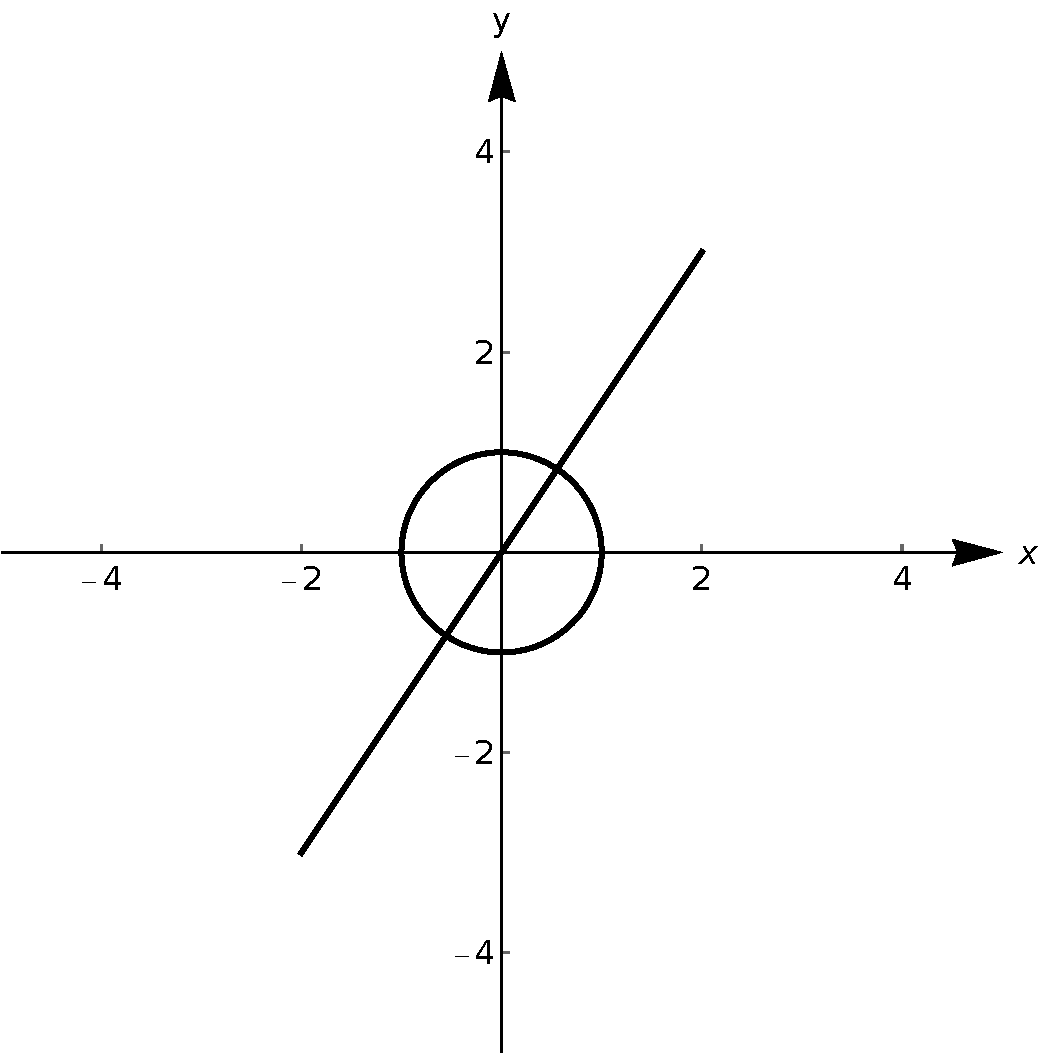
\includegraphics[width=0.3\textwidth]{fig_vector_fun_3a}}
\hspace{0.1cm}
\subfigure[\label{fig_vector_fun_3b}]{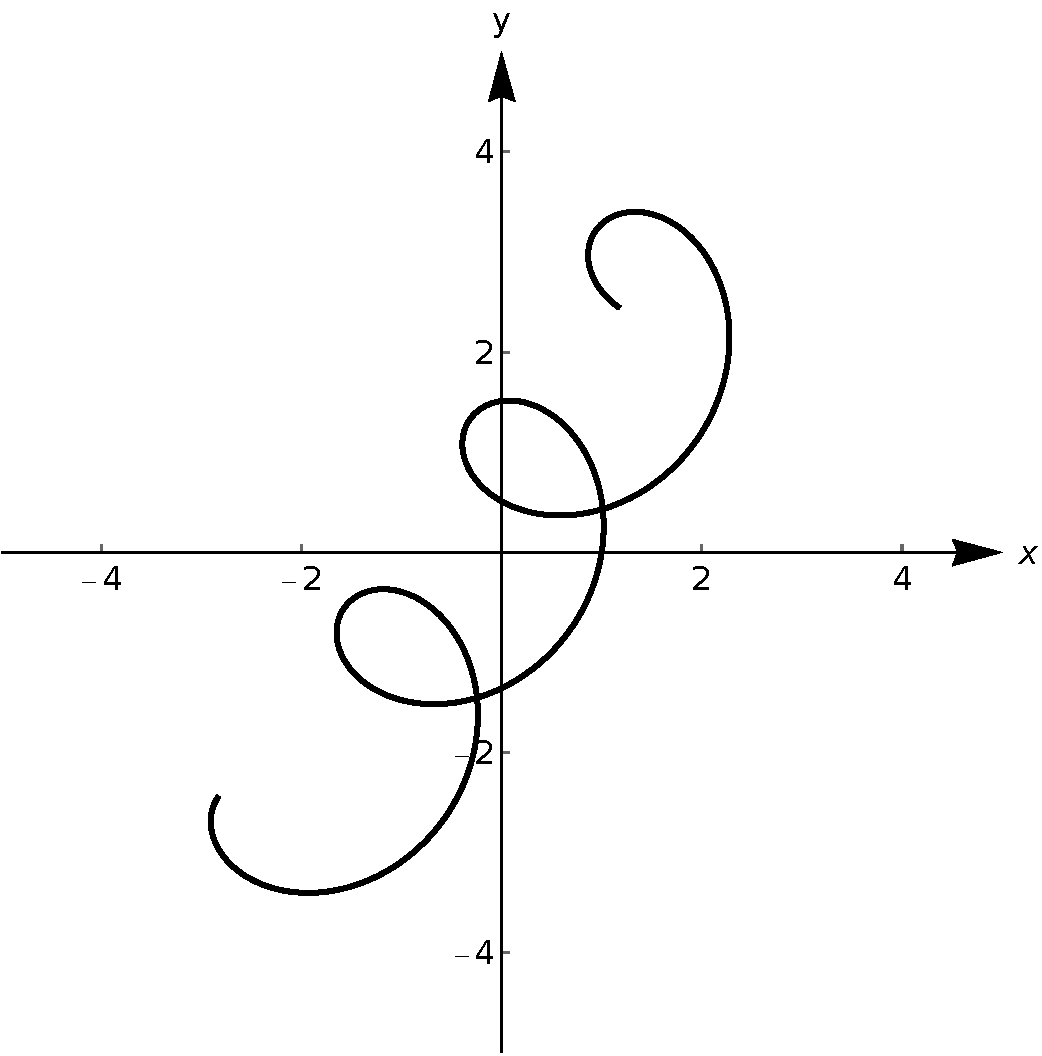
\includegraphics[width=0.3\textwidth]{fig_vector_fun_3b}}
\hspace{0.1cm}
\subfigure[\label{fig_vector_fun_3c}]{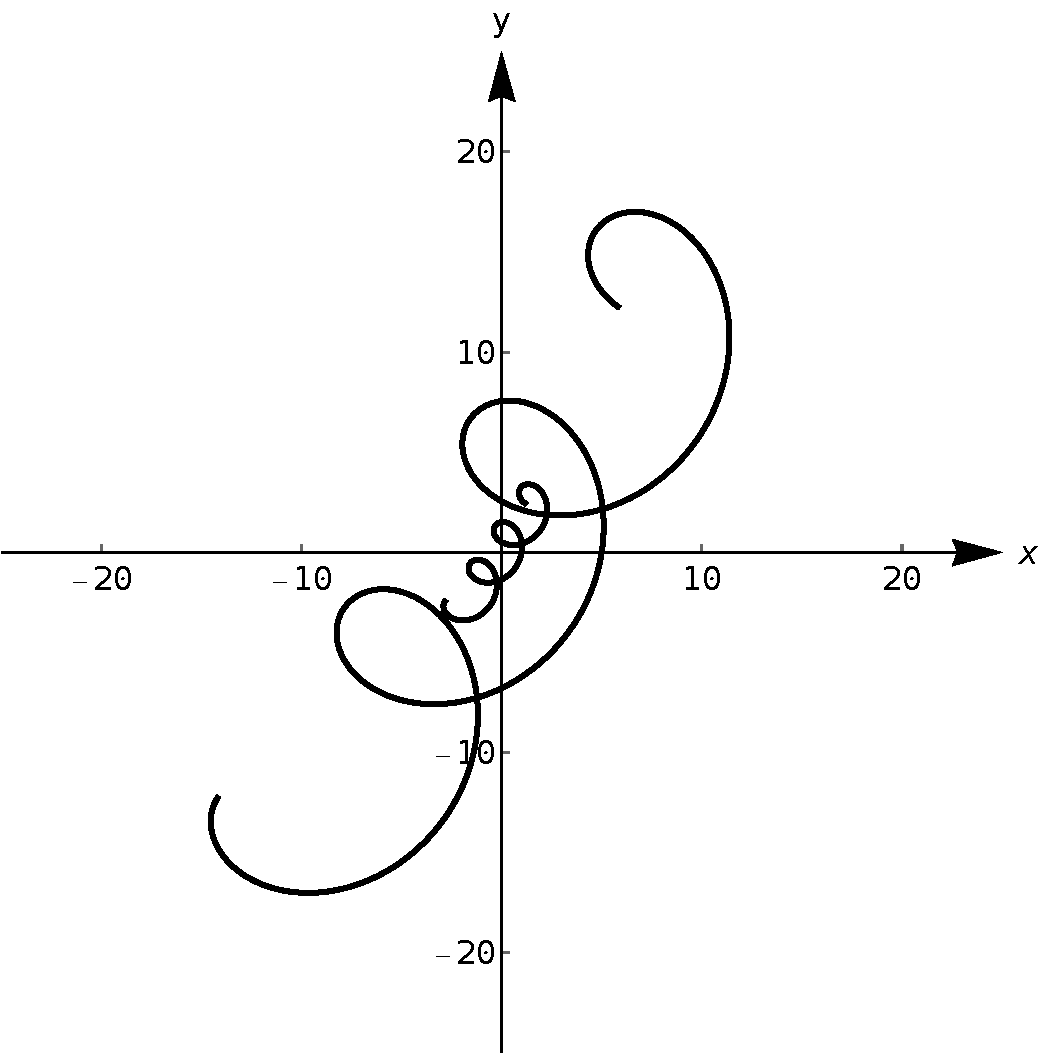
\includegraphics[width=0.3\textwidth]{fig_vector_fun_3c}}
}
\caption{Graphing the functions in Example \ref{ex_vvf3}.}
\end{figure}


Multiplying $\vec r(t)$ by 5 scales the function by 5, producing $5\vec r(t) =  \left( 5\cos (t)+1,5\sin (t)+1.5\right)$, which is graphed in Figure \ref{fig_vector_fun_3c} along with $\vec r(t)$. The new function is 5 times bigger than $\vec r(t)$. Note how the graph of $5\vec r(t)$ in (c) looks identical to the graph of $\vec r(t)$ in $(b)$. This is due to the fact that the $x$- and $y$- bounds of the plot in $(c)$ are exactly 5 times larger than the bounds in (b).
\end{example}


A vector--valued function $\vec r(t)$ is often used to describe the position of a moving object at time $t$. At $t=t_0$, the object is at $\vec r(t_0)$; at $t=t_1$, the object is at $\vec r(t_1)$. Knowing the locations $\vec r(t_0)$ and $\vec r(t_1)$ gives no indication of the path taken between them, but often we only care about the difference of the locations, $\vec r(t_1)-\vec r(t_0)$, the \textbf{displacement} (\textit{verplaatsing}).\index{displacement}

\begin{definition}[Displacement]\label{def:displacement}
Let $\vec r(t)$ be a vector--valued function and let $t_0<t_1$ be values in the domain. The \textbf{displacement} $\vec d$ of $\vec r$, from $t=t_0$ to $t=t_1$, is $$\vec d=\vec r(t_1)-\vec r(t_0).$$
\end{definition}

When the displacement vector is drawn with initial point at $\vec r(t_0)$, its terminal point is $\vec r(t_1)$. We think of it as the vector which points from a starting position to an ending position.

\begin{example}\label{ex_vvf5}
Let $\vec r(t) = \left( \cos \big(\frac{\pi}{2}t\big),\sin \big(\frac{\pi}2 t\big)\right)$. Graph $\vec r(t)$ on $-1\leq t\leq 1$, and find the displacement of $\vec r(t)$ on this interval.

\xhrulefill{gray}{2.5pt}Solution \xhrulefill{gray}{2.5pt}

The function $\vec r(t)$ traces out the unit circle, though at a different rate than the usual $\left( \cos (t),\sin (t)\right)$ parametrization. At $t_0=-1$, we have $\vec r(t_0) = \left( 0,-1\right)$; at $t_1=1$, we have $\vec r(t_1) = \left( 0,1\right)$. The displacement of $\vec r(t)$ on $[-1,1]$ is thus $\vec d = \left( 0,1\right) - \left( 0,-1\right) = \left( 0,2\right).$ A graph of $\vec r(t)$ on $[-1,1]$ is given in Figure \ref{fig_vector_fun_4}, along with the displacement vector $\vec d$ on this interval.

\begin{figure}[H]
	\begin{center}
			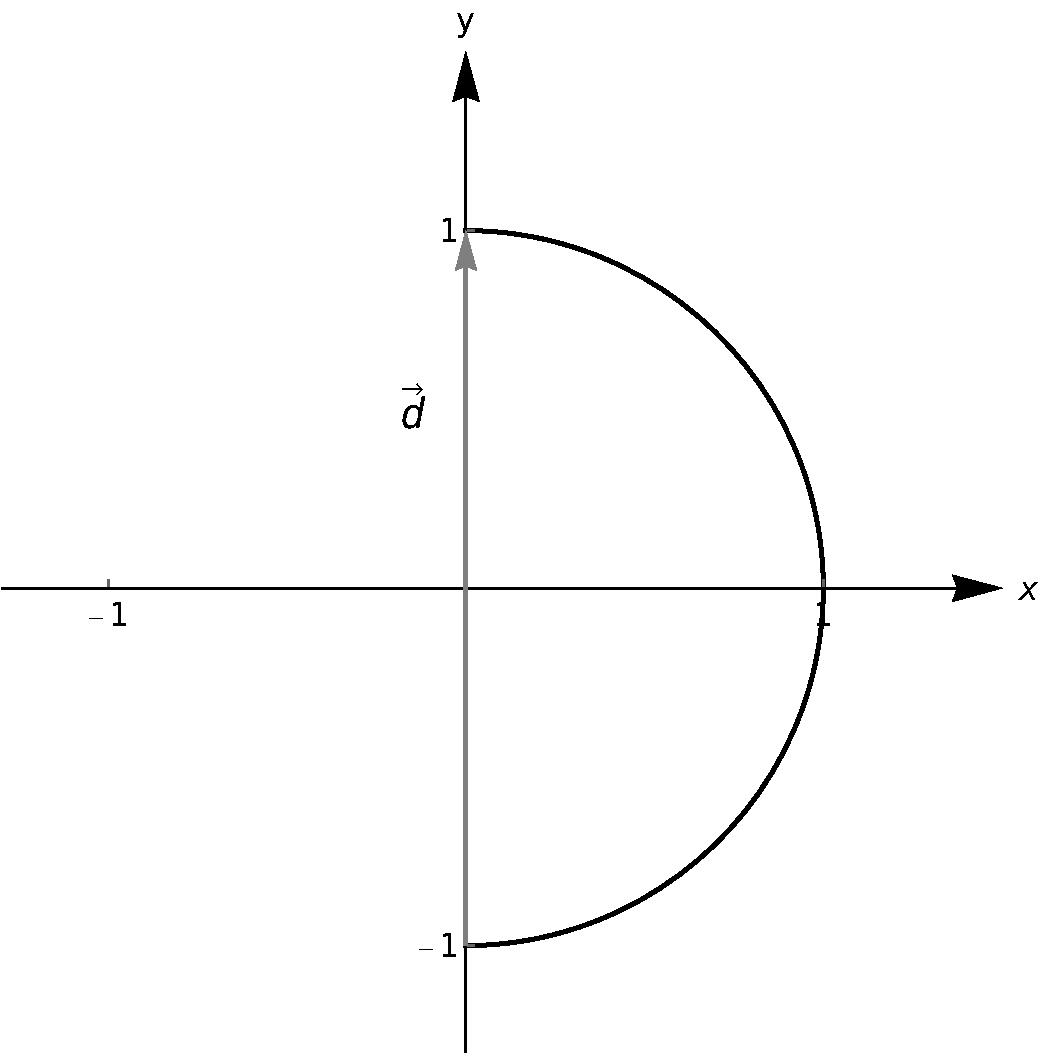
\includegraphics[width=0.35\textwidth]{fig_vector_fun_4}
	\caption{Graphing the displacement of a position function in Example \ref{ex_vvf5}.}
	\label{fig_vector_fun_4}
	\end{center}
\end{figure}


\end{example}

Measuring displacement makes us contemplate related, yet very different, concepts. Considering the semi--circular path the object in Example \ref{ex_vvf5} took, we can quickly verify that the object ended up a distance of 2 units from its initial location. That is, we can compute $\vnorm{d} = 2$. However, measuring distance from the starting point is different from measuring distance travelled. Being a semi--circle, we can measure the distance traveled by this object as $\pi\approx 3.14$ units. Knowing distance from the starting point allows us to compute average rate of change.

\begin{definition}[Average rate of change]\label{def:av_rate_of_change_vect}
Let $\vec r(t)$ be a vector--valued function, where each of its component functions is continuous on its domain, and let $t_0<t_1$. The \textbf{average rate of change of} $\vec r(t)$ on $[t_0,t_1]$ is
\index{average rate of change}
$$\text{average rate of change} = \frac{\vec r(t_1) - \vec r(t_0)}{t_1-t_0}.$$
\end{definition}

\begin{example}\label{ex_vvf6}
Let $\vec r(t) = \left( \cos\big(\frac{\pi}2t\big),\sin\big(\frac{\pi}2t\big)\right)$ as in Example \ref{ex_vvf5}. Find the average rate of change of $\vec r(t)$ on $[-1,1]$ and on $[-1,5]$.

\xhrulefill{gray}{2.5pt}Solution \xhrulefill{gray}{2.5pt}

We computed in Example \ref{ex_vvf5} that the displacement of $\vec r(t)$ on $[-1,1]$ was $\vec d = \left( 0,2\right)$. Thus the average rate of change of $\vec r(t)$ on $[-1,1]$ is:
$$\frac{\vec r(1) -\vec r(-1)}{1-(-1)} = \frac{\left( 0,2\right)}{2} = \left( 0,1\right).$$
We interpret this as follows: the object followed a semi--circular path, meaning it moved towards the right then moved back to the left, while climbing slowly, then quickly, then slowly again. On average, however, it progressed straight up at a constant rate of $\left( 0,1\right)$ per unit of time.
\end{example}

We considered average rates of change in Sections \ref{sec:limit_intro} and \ref{sec:derivative} as we studied limits and derivatives. The same is true here; in the following section we apply calculus concepts to vector--valued functions as we find limits, derivatives, and integrals. Understanding the average rate of change will give us an understanding of the derivative; displacement gives us one application of integration.

\section{Calculus and vector--valued functions}\label{sec:vvf_calc}

The previous section introduced us to a new mathematical object, the vector--valued function. We now apply calculus concepts to these functions. We start with the limit, then work our way through derivatives to integrals.

\subsection{Limits of vector-valued functions}

The initial definition of the limit of a vector--valued function is a bit intimidating, as was the definition of the limit in Definition \ref{def:limit}. The theorem following the definition shows that in practice, taking limits of vector--valued functions is no more difficult than taking limits of real--valued functions. Of course,  we can define one-sided limits in a manner very similar to Definition \ref{def:vvf_limit}.

\begin{definition}[Limits of vector--valued functions]\label{def:vvf_limit}
Let $I$ be an open interval containing $c$, and let $\vec r(t)$ be a vector--valued function defined on $I$, except possibly at $c$. %Let a vector--valued function $\vec r(t)$ be given, defined on an open interval $I$ containing $c$. 
The \textbf{limit of $\vec r(t)$} (\textit{limiet}), as $t$ approaches $c$, is $\vec L$, expressed as 
$$\lim_{t\to c} \vec r(t) = \vec L,$$ means that given any $\varepsilon>0$, there exists a $\delta>0$ such that for all $t\neq c$, if $|t-c| <\delta$, we have $\norm{\vec r(t) - \vec L} < \varepsilon.$
\index{vector--valued function!limits}\index{limit!of vector--valued functions}
\end{definition}

Note how the measurement of distance between real numbers is the absolute value of their difference; the measure of distance between vectors is the vector norm, or magnitude, of their difference.

The following theorem affirms that we can compute limits of vector--valued functions component--wise.

\ifcalculus
\begin{theorem}[Limits of vector-valued functions]\label{thm:vvf_limit}
\begin{enumerate}
	\item Let $\vec r(t) = \left( \,f(t),g(t)\,\right)$ be a vector--valued function in $\mathbb{R}^2$ defined on an open interval $I$ containing $c$, except possibly at $c$. Then
	\index{vector--valued function!limits}\index{limit!of vector--valued functions}\index[aut]{vectorfunctie ! limiet}
	$$\lim_{t\to c} \vec r(t) = \left( \lim_{t\to c}f(t)\, , \,\lim_{t\to c} g(t)\right).$$
	\item Let $\vec r(t) = \left( \,f(t),g(t),h(t)\,\right)$ be a vector--valued function in $\mathbb{R}^3$ defined on an open interval $I$ containing $c$, except possibly at $c$. Then 
	$$\lim_{t\to c} \vec r(t) = \left( \lim_{t\to c}f(t)\, , \,\lim_{t\to c} g(t)\,, \,\lim_{t\to c} h(t)\right).$$
\end{enumerate}
\end{theorem}
\fi


\ifanalysis
\begin{theorem}[Limits of vector-valued functions]\label{thm:vvf_limit}
Let $\vec r(t) = \left( \,f_1(t),f_2(t),\ldots,f_n(t)\,\right)$ be a $n$-dimensional vector--valued function in $\mathbb{R}^n$ defined on an open interval $I$ containing $c$, except possibly at $c$. Then
	$$\lim_{t\to c} \vec r(t) = \left( \lim_{t\to c}f_1(t)\,,\lim_{t\to c}f_2(t) ,\ldots, \,\lim_{t\to c} f_n(t)\right).$$
\end{theorem}
\fi

So, for instance, if 
\begin{equation}
\ds\vec r(t) = \left( \frac{\sin(t)}{t},\, t^2-3t+3,\,\cos(t)\right).
\label{vb_funvector}
\end{equation}
Then, $\ds \lim_{t\to 0}\vec r(t)$ is given by:
$$
\lim_{t\to0} \vec r(t) = \left( \lim_{t\to 0}\frac{\sin(t)}{t}\, , \, \lim_{t\to 0} (t^2-3t+3)\, , \, \lim_{t\to 0} \cos(t)\right)=\left( 1,3,1\right).
$$

\subsection{Continuity}
Having defined limits of vector--valued functions, it makes sense to explore the continuity of such functions. 


\begin{definition}[Continuity of vector--valued functions]\label{def:vvf_continuity}
Let $\vec r(t)$ be a vector--valued function defined on an open interval $I$ containing $c$.
\index{vector--valued function!continuity}
\begin{enumerate}
	\item $\vec r(t)$ is \textbf{continuous} at $c$ if $\ds \lim_{t\to c} \vec r(t) = \vec r(c)$.
	\item	If $\vec r(t)$ is continuous at all $c$ in $I$, then $\vec r(t)$ is continuous on $I$.
\end{enumerate}
\end{definition}

 Using one-sided limits, we can of course also define continuity on closed intervals as done before. Moreover, we again have a theorem that lets us evaluate continuity component--wise.

\begin{theorem}[Continuity of vector--valued functions]\label{thm:vvf_continuity}
Let $\vec r(t)$ be a vector--valued function defined on an open interval $I$ containing $c$. Then $\vec r(t)$ is continuous at $c$ if, and only if, each of its component functions is continuous at $c$.
\index{vector--valued function!continuity}\index[aut]{vectorfunctie ! continu\"iteit}
\end{theorem}

In the case of the vector--valued function defined by Equation~\eqref{vb_funvector}, for instance, $\vec r(t)$ is continuous at $t=1$ because each of the component functions is continuous at $t=1$. On the other hand, at $t=0$, the second and third components of $\vec r(t)$ are defined, but the first component, $(\sin (t))/t$, is not. Since the first component is not even defined at $t=0$, $\vec r(t)$ is not defined at $t=0$, and hence it is not continuous at $t=0$.

\subsection{Derivatives}
\subsubsection{Definition and properties}
Consider a vector--valued function $\vec r$ defined on an open interval $I$ containing $t_0$ and $t_1$. We can compute the displacement of $\vec r$ on $[t_0,t_1]$, as shown in Figure \ref{fig_vector_fun_5a}. Recall that dividing the displacement vector by $t_1-t_0$ gives the average rate of change on $[t_0,t_1]$, as shown in Figure~\ref{fig_vector_fun_5b}. 

\begin{figure}[h]
\centering
%\right)isebox{0.5cm}{
\centerline{
\subfigure[\label{fig_vector_fun_5a}]{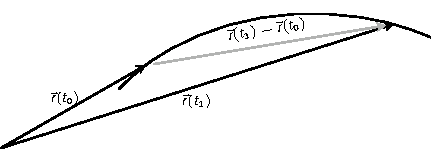
\includegraphics[width=0.43\textwidth]{fig_vector_fun_5a}}
\hspace{0.1cm}
\subfigure[\label{fig_vector_fun_5b}]{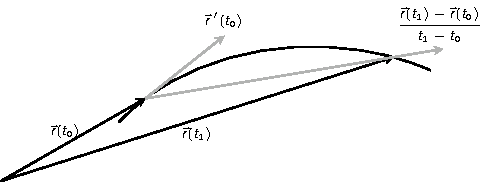
\includegraphics[width=0.43\textwidth]{fig_vector_fun_5b}}
}
\caption{Illustrating displacement, leading to an understanding of the derivative of vector--valued functions.}
\end{figure}

The \textbf{derivative} (\textit{afgeleide}) of a vector--valued function is a measure of the instantaneous rate of change, measured by taking the limit as the length of $[t_0,t_1]$ goes to 0. Instead of thinking of an interval as $[t_0,t_1]$, we think of it as $[c,c+h]$ for some value of $h$ (hence the interval has length $h$).  The average rate of change is 
$$\frac{\vec r(c+h)-\vec r(c)}{h}$$ for any value of $h\neq0$. We take the limit as $h\to0$ to measure the instantaneous rate of change; this is the derivative of $\vec r$.

%We begin with a definition of the derivative that is very similar to Definition \ref{def:the_derivative}.

\begin{definition}[Derivative of a vector--valued function]\label{def:vvf_derivative}
Let $\vec r(t)$ be continuous on an open interval $I$ containing $c$.
\index{vector--valued function!derivative}\index{derivative!vector--valued functions}\index[aut]{vectorfunctie ! afgeleide}
\begin{enumerate}
	\item The \textbf{derivative of $\vec r$ at $t=c$} is
	$$ \vrp (c) = \lim_{h\to 0} \frac{\vec r(c+h) - \vec r(c)}{h}.$$
	\item	The \textbf{derivative of $\vec r$} is
	$$ \vrp (t) = \lim_{h\to 0} \frac{\vec r(t+h) - \vec r(t)}{h}.$$
\end{enumerate}
\end{definition}

Alternate notations for the derivative of $\vec r$ include: $$\vrp(t) = \frac{d}{dt}\big(\,\vec r(t)\,\big) = \frac{d\vec r}{dt}.$$




If a vector--valued function  has a derivative for all $c$ in an open interval $I$, we say that $\vec r(t)$ is \textbf{differentiable} (\textit{afleidbaar}) on $I$. Again, of course,  using one-sided limits, we can define differentiability on closed intervals. We might view Definition~\ref{def:vvf_derivative} as intimidating, but recall that we can evaluate limits component--wise. The following theorem verifies that this means we can compute derivatives component--wise as well, making the task not too difficult.

\ifcalculus
\begin{theorem}[Derivative of a vector--valued function]\label{thm:vvf_deriv}
\begin{enumerate}
	\item Let $\vec r(t) = \left( \, f(t), g(t)\,\right)$. Then 
	$$\vrp(t) = \left( \fp(t), g'(t)\, \right).$$
	\item Let $\vec r(t) = \left( \, f(t), g(t), h(t)\,\right)$. Then
	\index{vector--valued function!derivatives}\index{derivative!vector--valued functions}\index[aut]{vectorfunctie ! afgeleide}
	$$\vrp(t) = \left( \fp(t), g'(t), h'(t)\, \right).$$
\end{enumerate}
\end{theorem}
\fi

\ifanalysis

\begin{theorem}[Derivative of a vector--valued function]\label{thm:vvf_deriv}
Let $\vec r(t) = \left( \, f_1(t),f_2(t),\ldots, f_n(t)\,\right)$. Then 
	$$\vrp(t) = \left( f_1'(t),f_2'(t),\ldots, f_n'(t)\, \right).$$
	\index{vector--valued function!derivatives}\index{derivative!vector--valued functions}\index[aut]{vectorfunctie ! afgeleide}
\end{theorem}


\begin{proof}

This theorem follows easily by combining Definition~\ref{thm:vvf_deriv} and vector arithmetic (Section~\ref{sec_vector_arith}). For instance, for a three-dimensional vector-valued function $\vec r(t) = \left( \, f(t), g(t), h(t)\,\right)$, we get: 
\begin{eqnarray*}
  {\vec r}'(t)&=&\lim_{\Delta t\to0}{{\vec r}(t+\Delta t)-{\vec r}(t)\over
  \Delta t}\\[0.2cm]
  &=&\lim_{\Delta t\to0}{\left( f(t+\Delta t)-f(t),g(t+\Delta t)-g(t),
  h(t+\Delta t)-h(t)\right)\over \Delta t}\\[0.2cm]
  &=&\lim_{\Delta t\to0}\left(  {f(t+\Delta t)-f(t)\over\Delta t},
  {g(t+\Delta t)-g(t)\over\Delta t},
  {h(t+\Delta t)-h(t)\over \Delta t}\right)\\[0.2cm]
  &=&\left(  f'(t),g'(t),h'(t)\right)
\end{eqnarray*}


\end{proof}

\fi


\begin{example}\label{ex_vvflimit3}
Let $\vec r(t) = \left( t^2,t\right)$. 
\begin{enumerate}
	\item Sketch $\vec r(t)$ and $\vrp(t)$ on the same axes.
	\item	Compute $\vrp(1)$ and sketch this vector with its initial point at the origin and at $\vec r(1)$.
\end{enumerate}

\xhrulefill{gray}{2.5pt}Solution \xhrulefill{gray}{2.5pt}


\begin{enumerate}
\item	Theorem \ref{thm:vvf_deriv} allows us to compute derivatives component--wise, so
$$\vrp(t) = \left( 2t, 1\right).$$ $\vec r(t)$ and $\vrp(t)$ are graphed together in Figure \ref{fig_vector_fun_6a}. Note how plotting the two of these together, in this way, is not very illuminating. When dealing with real--valued functions, plotting $f(x)$ with $\fp(x)$ gave us useful information as we were able to compare $f$ and $\fp$ at the same $x$-values. When dealing with vector--valued functions, it is hard to tell which points on the graph of $\vrp$ correspond to which points on the graph of $\vec r$.

\item	We easily compute $\vrp(1) = \left( 2,1\right)$, which is drawn in Figure \ref{fig_vector_fun_6b} with its initial point at the origin, as well as at $\vec r(1) = \left( 1,1\right).$ These are sketched in Figure \ref{fig_vector_fun_6b}.


\begin{figure}[H]
\centering
%\right)isebox{0.5cm}{
\centerline{
\subfigure[\label{fig_vector_fun_6a}]{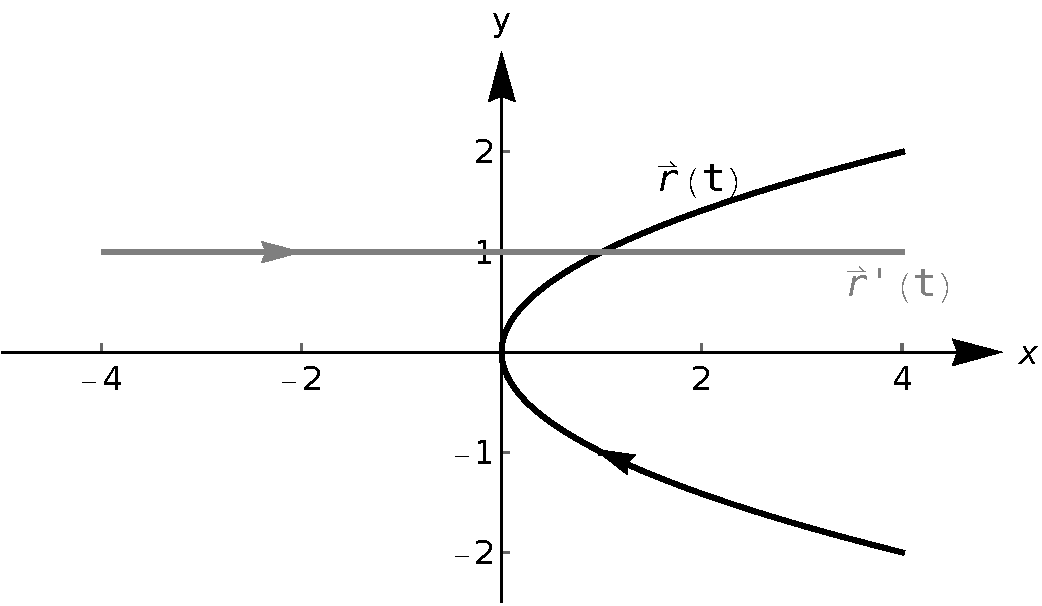
\includegraphics[width=0.43\textwidth]{fig_vector_fun_6a}}
\hspace{0.1cm}
\subfigure[\label{fig_vector_fun_6b}]{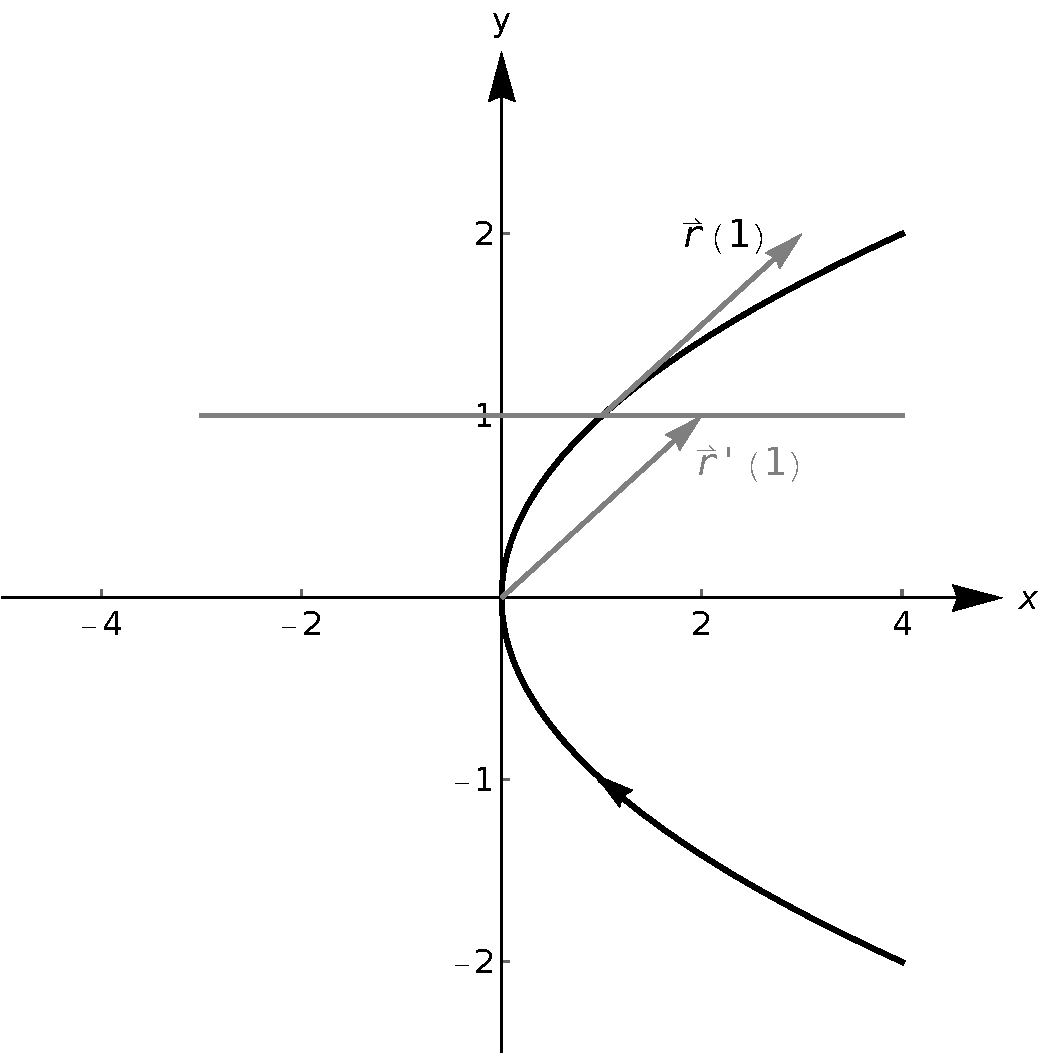
\includegraphics[width=0.35\textwidth]{fig_vector_fun_6b}}
}
\caption{Graphing the derivative of a vector--valued function in Example \ref{ex_vvflimit3}.}
\end{figure}


\end{enumerate}
\end{example}

Having established derivatives of vector--valued functions, we now explore the relationships between the derivative and other vector operations. The following properties show how the derivative interacts with vector addition and the various vector products. For that purpose, let $\vec r$ and $\vec s$ be differentiable vector--valued functions, let $f$ be a differentiable real--valued function, and let $c$ be a real number. Then the following properties hold. 

\begin{multicols}{2}
\begin{itemize}
	\item $\ds \frac{d}{dt}\Big(\vec r(t) \pm \vec s(t)\Big) = \vrp(t) \pm \vec s\,'(t)$
	\item $\ds \frac{d}{dt}\Big(c\vec r(t)\Big) = c\vrp(t)$
	\item $\ds \frac{d}{dt}\Big(f(t)\vec r(t)\Big) = \fp(t)\vec r(t) + f(t)\vrp(t)$
	\item $\ds \frac{d}{dt}\Big(\vec r(t)\cdot \vec s(t) \Big) = \vrp(t)\cdot \vec s(t) + \vec r(t)\cdot \vec s\,'(t)$
	\item $\ds \frac{d}{dt}\Big(\vec r(t)\times \vec s(t) \Big) = \vrp(t)\times \vec s(t) + \vec r(t)\times \vec s\,'(t)$
	\item $\ds \frac{d}{dt}\Big(\vec r\big(f(t)\big)\Big) = \vrp\big(f(t)\big)\fp(t)$
	\end{itemize}
\end{multicols}	
	
\begin{example}\label{ex_vvfderiv2}
Let $\vec r(t) = \left( t, t^2-1\right)$ and let $\vec u(t)$ be the unit vector that points in the direction of $\vec r(t)$.
\begin{enumerate}
	\item Graph $\vec r(t)$ and $\vec u(t)$ on the same axes, on $[-2,2]$.
	\item	Find $\vec u\,'(t)$ and sketch $\vec u\,'(-2)$, $\vec u\,'(-1)$ and $\vec u\,'(0)$. Sketch each with initial point the corresponding point on the graph of $\vec u$.
\end{enumerate}

\xhrulefill{gray}{2.5pt}Solution \xhrulefill{gray}{2.5pt}


\begin{enumerate}
	\item To form the unit vector that points in the direction of $\vec r$, we need to divide $\vec r(t)$ by its magnitude. 
	$$\norm{\vec r(t)} = \sqrt{t^2+(t^2-1)^2} \quad \Rightarrow \quad \vec u(t) = \frac{1}{\sqrt{t^2+(t^2-1)^2}}\vec r(t)$$
	
	$\vec r(t)$ and $\vec u(t)$ are graphed in Figure \ref{fig_vector_fun_7a}. Note how the graph of $\vec u(t)$ forms part of a circle; this must be the case, as the length of $\vec u(t)$ is 1 for all $t$.

	%\drawexampleline
	
	\item To compute $\vec u\,'(t)$, we rely on the above properties and write $$\vec u(t) = f(t)\vec r(t),\quad  \text{where}\quad f(t) = \frac{1}{\sqrt{t^2+(t^2-1)^2}}=\big(t^2+(t^2-1)^2\big)^{-1/2}.$$ 
	
We find $\fp(t)$ using the chain rule:
\begin{align*}
\fp(t) &= -\frac12\big(t^2+(t^2-1)^2\big)^{-3/2}\big(2t+2(t^2-1)(2t)\big)\\[0.2cm]
			&= -\frac{2t(2t^2-1)}{2\big(\sqrt{t^2+(t^2-1)^2}\,\big)^3}.
\end{align*}
We now find $\vec u\,'(t)$:
\begin{align*}
\vec u\,'(t) &=  \fp(t)\vec u(t) + f(t)\vec u\,'(t) \\[0.2cm]
				&=  -\frac{2t(2t^2-1)}{2\big(\sqrt{t^2+(t^2-1)^2}\,\big)^3}\left( t,t^2-1\right) + \frac{1}{\sqrt{t^2+(t^2-1)^2}}\left( 1,2t\right).
\end{align*}
 We can use this formula to compute $\vec u\,'(-2)$, $\vec u\,'(-1)$ and $\vec u\,'(0)$:
\begin{align*}
\vec u\,'(-2) &= \left(-\frac{15}{13 \sqrt{13}},-\frac{10}{13
   \sqrt{13}}\right) \approx \left( -0.320,-0.213\right),\\[0.2cm]
\vec u\,'(-1) &= \left( 0,-2\right),\\
\vec u\,'(0) &= \left( 1,0\right).
\end{align*}

Each of these is sketched in Figure \ref{fig_vector_fun_7b}. Note how the length of the vector gives an indication of how quickly the circle is being traced at that point. When $t=-2$, the circle is being drawn relatively slow; when $t=-1$, the circle is being traced much more quickly.
\end{enumerate}

\begin{figure}[H]
\centering
%\right)isebox{0.5cm}{
\centerline{
\subfigure[\label{fig_vector_fun_7a}]{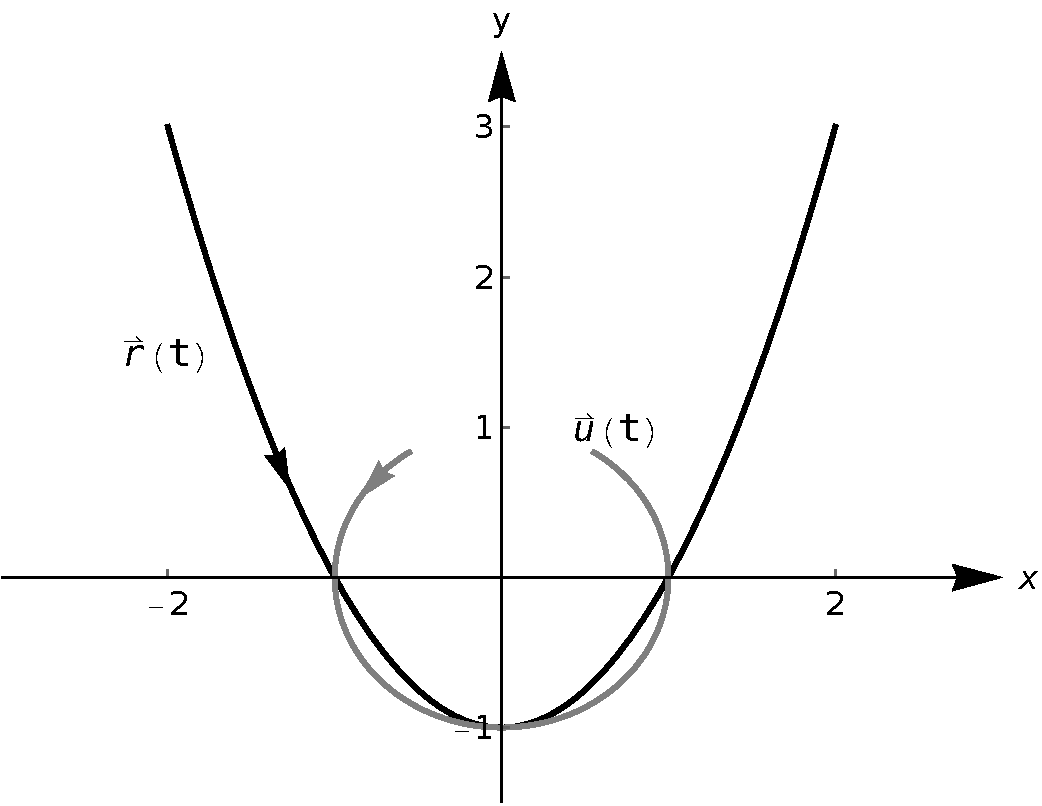
\includegraphics[width=0.43\textwidth]{fig_vector_fun_7a}}
\hspace{0.1cm}
\subfigure[\label{fig_vector_fun_7b}]{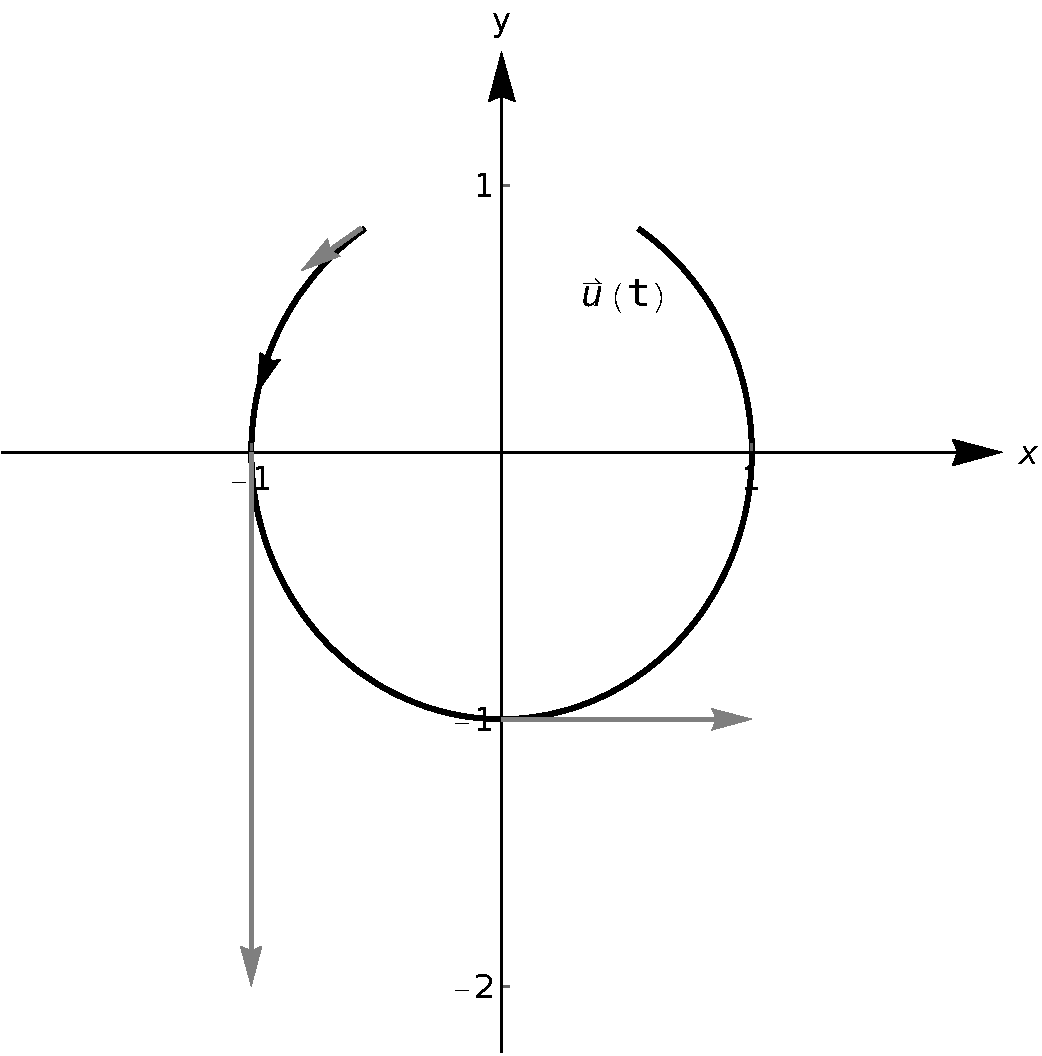
\includegraphics[width=0.43\textwidth]{fig_vector_fun_7b}}
}
\caption{Graphing $\vec r(t)$ and $\vec u(t)$ (a) and some of the derivatives of $\vec u(t)$ (b) in Example \ref{ex_vvfderiv2}.}
\end{figure}

\end{example}


\subsubsection{Tangent vector and lines}
In Example \ref{ex_vvflimit3}, sketching a particular derivative with its initial point at the origin did not seem to reveal anything significant. However, when we sketched the vector with its initial point on the corresponding point on the graph, we did see something significant: the vector appeared to be tangent to the graph. We have not yet defined what tangent means in terms of curves in space; in fact, we use the derivative to define this term.


\begin{definition}[Tangent vector and line]\label{def:vector_tangent}
Let $\vec r(t)$ be a differentiable vector--valued function on an open interval $I$ containing $c$, where \linebreak $\vrp(c)\neq \vec 0$.
\index{tangent line}\index{vector--valued function!tangent line}\index[aut]{vectorfunctie ! raaklijn}
\begin{enumerate}
	\item A vector $\vec v$ is \textbf{tangent} (\textit{rakend}) to the graph of $\vec r(t)$ at $t=c$ if $\vec v$ is parallel to $\vrp(c)$.
	\item	The tangent line  to the graph of $\vec r(t)$ at $t=c$ is the line through $\vec r(c)$ with direction parallel to $\vrp(c)$. An equation of the \textbf{tangent line} (\textit{raaklijn}) is 
	$$\vec y=\vec \ell(t) = \vec r(c) + t\,\vrp(c).$$
\end{enumerate}
\end{definition}


\begin{example}\label{ex_vvfderiv3}
Find the equations of the lines tangent to $\vec r(t) = \left( t^3,t^2\right)$ at $t=-1$ and $t=0$.

\ifcalculus\pagebreak\fi
\xhrulefill{gray}{2.5pt}Solution \xhrulefill{gray}{2.5pt}

We find that $\vrp(t) = \left( 3t^2,2t\right)$. At $t=-1$, we have
$$\vec r(-1) = \left( -1,1\right)\quad \text{and}\quad \vrp(-1) = \left( 3,-2\right),$$
so the equation of the line tangent to the graph of $\vec r(t)$ at $t=-1$ is
$$\vec \ell(t) = \left( -1,1\right) + t\left( 3,-2\right).$$ This line is graphed with $\vec r(t)$ in Figure \ref{fig_vector_fun_8}.

At $t=0$, we have $\vrp(0) = \left( 0,0\right)=\vec 0$! This implies that the tangent line has no direction. We cannot apply Definition \ref{def:vector_tangent}, hence cannot find the equation of the tangent line.



\begin{figure}[H]\
	\begin{center}
			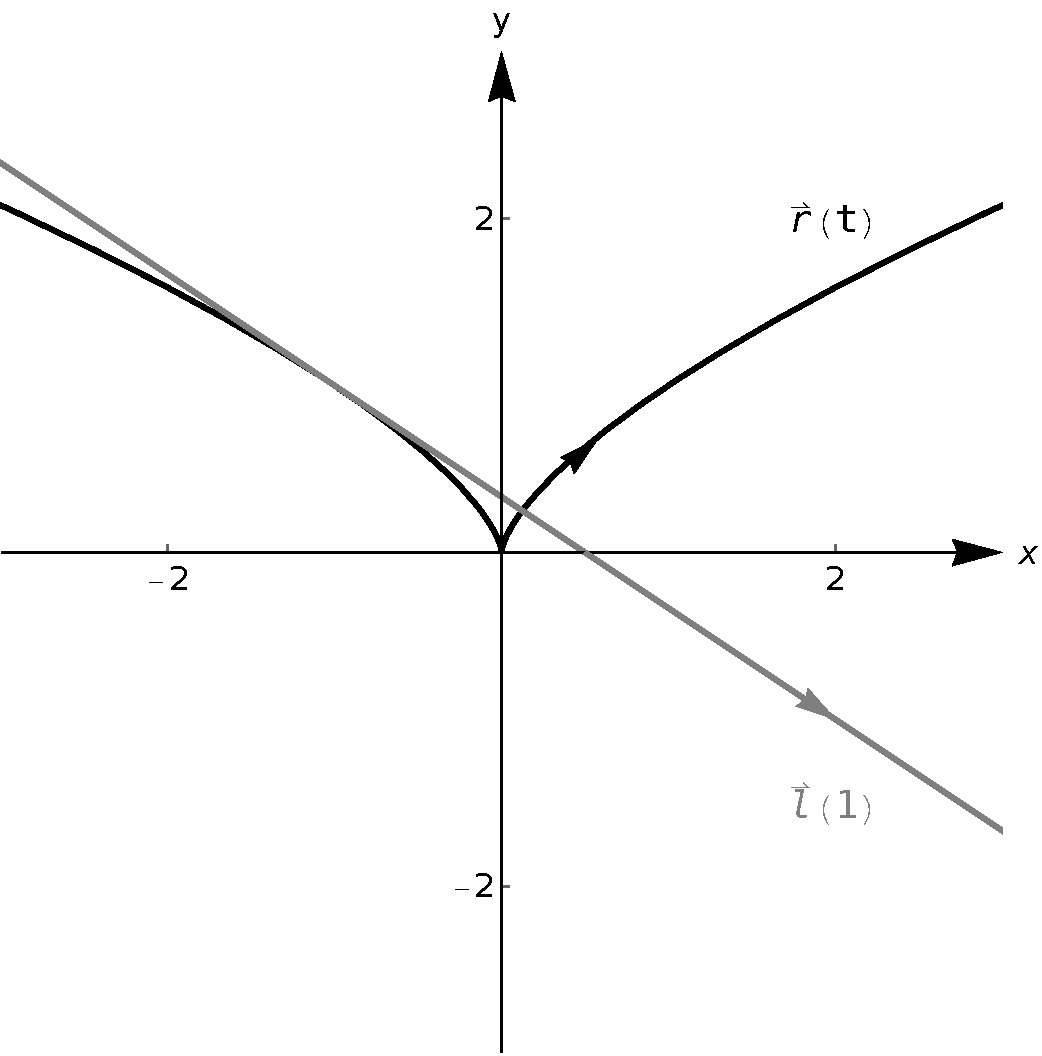
\includegraphics[width=0.35\textwidth]{fig_vector_fun_8}
	\caption{Graphing $\vec r(t)$ and its tangent line in Example \ref{ex_vvfderiv3}.}
	\label{fig_vector_fun_8}
	\end{center}
\end{figure}


\end{example}

\subsubsection{Smoothness}

We were unable to compute the equation of the tangent line to $\vec r(t)= \left( t^3,t^2\right)$ at $t=0$ because \\ $\vrp(0) = \vec 0$. The graph in Figure \ref{fig_vector_fun_8} shows that there is a cusp at this point. This leads us to another definition of \textbf{smooth} (\textit{glad}), previously defined by Definition \ref{def:smooth}.

\begin{definition}[Smooth vector--valued function]\label{def:vector_smooth}
Let $\vec r(t)$ be a differentiable vector--valued function on an open interval $I$ where $\vrp(t)$ is continuous on $I$. $\vec r(t)$ is \textbf{smooth} on $I$ if $\vrp(t)\neq \vec 0$ on $I$.
\index{smooth}\index{vector--valued function!smooth}\index[aut]{vectorfunctie ! glad}
\end{definition}


It is a basic geometric fact that a line tangent to a circle at a point $P$ is perpendicular to the line passing through the center of the circle and $P$. This is illustrated in Figure \ref{fig_vector_fun_7b}; each tangent vector is perpendicular to the line that passes through its initial point and the centre of the circle. Since the centre of the circle is the origin, we can state this another way: $\vec u\,'(t)$ is orthogonal to $\vec u(t)$.

Recall that the dot product serves as a test for orthogonality: if $\vec u\cdot \vec v = 0$, then $\vec u$ is orthogonal to $\vec v$. Thus in the above example, $\vec u(t)\cdot \vec u\,'(t)=0$. This is true for any vector--valued function that has a constant length, that is, that traces out part of a circle. It has important implications later on, so we state it as a theorem.

\begin{theorem}[Vector--valued functions of constant length]\label{thm:vects_of_constant_length}
Let $\vec r(t)$ be a  vector--valued function of constant length that is differentiable on an open interval $I$. That is, $\norm{\vec r(t)} = c$ for all $t$ in $I$. Then $\vec r(t)\cdot\vrp(t) = 0$ for all $t$ in $I$.
\end{theorem}

\subsection{Integration}
Before formally defining integrals of vector--valued functions, consider the following equation that our calculus experience tells us should be true:
$$\int\limits_a^b \vrp(t)\ dt = \vec r(b) - \vec r(a).$$
That is, the integral of a rate of change function should give total change. In the context of vector--valued functions, this total change is displacement. The above equation is true; we now develop the theory to show why.

We can define antiderivatives and the indefinite integral of vector--valued functions in the same manner we defined indefinite integrals in Definition~\ref{def:antider}. However, we cannot define the definite integral of a vector--valued function as we did in Definition \ref{def:def_int}. That definition was based on the signed area between a function $y=f(x)$ and the $x$-axis. An area--based definition will not be useful in the context of vector--valued functions.
Instead, we define the definite integral of a vector--valued function in a manner similar to that of Theorem \ref{thm:riemann_sum}, utilizing Riemann sums. 

\begin{definition}[Antiderivatives, integrals of vector--valued functions]\label{def:vvf_integral}
Let $\vec r(t)$ be a continuous vector--valued function on $[a,b]$. An \textbf{antiderivative of $\vec r(t)$} (\textit{primitieve functie}) is a function $\vec R(t)$ such that $\vec R'(t) = \vec r(t)$.\\

The set of all antiderivatives of $\vec r(t)$ is the \textbf{indefinite integral of $\vec r(t)$} (\textit{onbepaalde integraal}), denoted by 
$$\int \vec r(t)\ dt.$$

The \textbf{definite integral  of $\vec r(t)$} (\textit{bepaalde integraal}) on $[a,b]$ is 
$$\int\limits_a^b \vec r(t)\ dt =\lim_{\mathcal{T}\to 0} \sum_{i=1}^n\vec r(c_i)\Delta t_i,$$ where $\Delta t_i$ is the length of the $i^{\,\text{th}}$ subinterval of a partition of $[a,b]$, $\mathcal{T}$ is the length of the largest subinterval in the partition, and $c_i$ is any value in the $i^{\,\text{th}}$ subinterval of the partition.%
\index{antiderivative!of vector--valued function}\index[aut]{vectorfunctie ! primitieve}
\index{definite integral!of vector--valued function}\index[aut]{vectorfunctie ! bepaalde integraal}
\index{indefinite integral!of vector--valued function}\index[aut]{vectorfunctie ! onbepaalde integraal}
\index{integration!of vector--valued function}\index[aut]{vectorfunctie ! integratie}
\end{definition}

It is probably difficult to infer meaning from the definition of the definite integral. The important thing to realize from the definition is that it is built upon limits, which we can evaluate component--wise.  The following theorem simplifies the computation of definite integrals.

\ifcalculus
\pagebreak
\begin{theorem}[Indefinite and definite integrals of vector--valued functions]\label{thm:vvf_integration}
Let $\vec r(t) = \left( f(t),g(t)\right)$ be a vector--valued function in $\mathbb{R}^2$ that are continuous on $[a,b]$.
\begin{enumerate}
	\item $\ds \int \vec r(t)\ dt = \left( \int f(t)\ dt, \int g(t)\ dt\right)$
	\item	$\ds \int\limits_a^b \vec r(t)\ dt = \left( \int\limits_a^b f(t)\ dt, \int\limits_a^b g(t)\ dt\right)$
\end{enumerate}
A similar statement holds for vector--valued functions in $\mathbb{R}^3$.
\index{vector--valued function!integration}\index{integration!of vector--valued functions}
\end{theorem}
\fi

\ifanalysis
\begin{theorem}[Indefinite and definite integrals of vector--valued functions]\label{thm:vvf_integration}
Let $\vec r(t) = \left( f_1(t),f_2(t),\ldots,f_n(t)\right)$ be a vector--valued function in $\mathbb{R}^n$ that is continuous on $[a,b]$.
\begin{enumerate}
	\item $\ds \int \vec r(t)\ dt = \left( \int f_1(t)\ dt,\int f_2(t)\ dt,\ldots, \int f_n(t)\ dt\right)$
	\item	$\ds \int\limits_a^b \vec r(t)\ dt = \left( \int\limits_a^b f_1(t)\ dt,\int\limits_a^b f_2(t)\ dt,\ldots, \int\limits_a^b f_n(t)\ dt\right)$
\end{enumerate}
\index{vector--valued function!integration}\index{integration!of vector--valued functions}
\end{theorem}
\fi



\ifanalysis

\begin{proof}
This theorem is an immediate consequence of our understanding of the derivative of a vector function through Theorem~\ref{thm:vvf_deriv}.
\end{proof}

\fi




\begin{example}\label{ex_vvfint1}
Let $\vec r(t) = \left( e^{2t},\sin(t)\right)$. Evaluate $$\ds \int\limits_0^1 \vec r(t) \ dt.$$


\xhrulefill{gray}{2.5pt}Solution \xhrulefill{gray}{2.5pt}

We follow Theorem \ref{thm:vvf_integration}.
\allowdisplaybreaks
\begin{align*}
\int\limits_0^1 \vec r(t) \ dt &= \int\limits_0^1 \left( e^{2t},\sin(t)\right) \ dt \\[0.2cm]
				&= \left( \int\limits_0^1 e^{2t}\ dt\ , \int\limits_0^1 \sin(t) \ dt \right) \\[0.2cm]
				&= \left( \frac12e^{2t}\Big|_0^1\ , (-\cos(t)) \Big|_0^1\right) \\[0.2cm]
				&= \left( \frac12(e^2-1)\ , -\cos(1)+1\right)\\[0.2cm]
				&\approx \left( 3.19,0.460\right)
\end{align*}
\end{example}

What does the integration of a vector--valued function mean? There are many applications, but none as direct as the area under the curve that we used in understanding the integral of a real--valued function. A key understanding for us comes from considering the integral of a derivative: 
$$\int\limits_a^b \vrp(t)\ dt = \vec r(t)\Big|_a^b = \vec r(b)-\vec r(a).$$ This indicates integrating a rate of change function gives displacement.\index{displacement}

Noting that vector--valued functions are closely related to parametric equations, we can describe the arc length of the graph of a vector--valued function as an integral. Given parametric equations $x=f(t)$, $y=g(t)$, the arc length on $[a,b]$ of the graph is
$$L = \int\limits_a^b\sqrt{\fp(t)^2+g'(t)^2}\ dt,$$
as stated in Theorem \ref{thm:arc_length_parametric}. %in Section \ref{sec:par_calc}. 
If $\vrt = \left( f(t), g(t)\right)$, note that $\sqrt{\fp(t)^2+g'(t)^2} = \norm{\vrp(t)}$. Therefore we can express the arc length of the graph of a vector--valued function as an integral of the magnitude of its derivative.

\begin{theorem}[Arc length of a vector--valued function]\label{thm:vvf_arc_length}
Let \vrt\ be a vector--valued function where $\vrp(t)$ is continuous on $[a,b]$. The \textbf{arc length} (\textit{booglengte}) $L$ of the graph of \vrt\ is 
\index{vector--valued function!arc length}\index{arc length}\index[aut]{vectorfunctie ! booglengte}
$$L = \int\limits_a^b \norm{\vrp(t)}\ dt.$$
\end{theorem}

Note that we are actually integrating a scalar function here, not a vector--valued function.

The remainder of this section takes what we have established thus far and applies it to objects in motion. 

\subsection{The calculus of motion}\label{sec:vvf_motion}

A common use of vector--valued functions is to describe the motion of an object in the plane or in space. A position function $\vec r(t)$ gives the position of an object at time $t$. This section explores how derivatives and integrals are used to study the motion described by such a function.

\begin{definition}[Velocity, speed and acceleration]\label{def:vvf_motion}
Let $\vec r(t)$ be a position function in $\mathbb{R}^2$ or $\mathbb{R}^3$.
\begin{enumerate}
	\item \textbf{Velocity}, denoted $\vec v(t)$, is the instantaneous rate of position change; that is, $\vec v(t) = \vrp(t)$.
	\item	\textbf{Speed} is the magnitude of velocity, $\norm{\vec v(t)}$.
	\item	\textbf{Acceleration}, denoted $\vec a(t)$, is the instantaneous rate of velocity change; that is, \linebreak$\vec a(t) = \vec v\,'(t) = \vrp'(t)$.
	\index{velocity}\index{speed}\index{acceleration}\index[aut]{snelheid}\index[aut]{versnelling}
\end{enumerate}
\end{definition}

\begin{example}\label{ex_motion1}
An object is moving with position function $\vec r(t) = \left( t^2-t,t^2+t\right)$, $-3\leq t\leq 3$, where distances are measured in metres and time is measured in seconds.
\begin{enumerate}
	\item Find \vvt\  and \vat.
	\item	Sketch \vrt; plot $\vec v(-1)$, $\vec a(-1)$, $\vec v(1)$ and $\vec a(1)$, each with their initial point at their corresponding point on the graph of $\vrt$.
	\item	When is the object's speed minimized?
\end{enumerate}

\ifcalculus\pagebreak\fi
\xhrulefill{gray}{2.5pt}Solution \xhrulefill{gray}{2.5pt}

\begin{enumerate}
	\item Taking derivatives, we find
	$$\vvt = \vrp(t) =\left( 2t-1,2t+1\right) \quad \text{and} \quad \vat = \vrp'(t) = \left( 2,2\right).$$
	Note that the acceleration is constant.
	
	\item		$\vec v(-1) = \left( -3,-1\right)$,\ \ $\vec a(-1) = \left( 2,2\right)$; \quad $\vec v(1) = \left( 1,3\right)$,\ \ $\vec a(1) = \left( 2,2\right)$. These are plotted with \vrt\ in Figure \ref{fig_vector_fun_9a}.
	
	We can think of acceleration as pulling the velocity vector in a certain direction. At $t=-1$, the velocity vector points down and to the left; at $t=1$, the velocity vector has been pulled in the $\left( 2,2\right)$ direction and is now pointing up and to the right. In Figure \ref{fig_vector_fun_9b} we plot more velocity/acceleration vectors, making more clear the effect acceleration has on velocity.
	
	Since $\vat$ is constant in this example, as $t$ grows large \vvt\ becomes almost parallel to \vat. For instance, when $t=10$, $\vec v(10) = \left( 19,21\right)$, which is nearly parallel to $\left( 2,2\right)$.
	
	\item		The object's speed is given by 
	$$\norm{\vvt} = \sqrt{(2t-1)^2+(2t+1)^2} =\sqrt{8t^2+2}.$$ To find the minimal speed, we could apply calculus techniques (such as set the derivative equal to 0 and solve for $t$, etc.) but we can find it by inspection. Inside the square root we have a quadratic which is minimized when $t=0$. Thus the speed is minimized at $t=0$, with a speed of $\sqrt{2}$ m/s.
	
	The graph in Figure \ref{fig_vector_fun_9b} also implies speed is minimized here. The filled dots on the graph are located at integer values of $t$ between $-3$ and 3. Dots that are far apart imply the object travelled a far distance in 1 second, indicating high speed; dots that are close together imply the object did not travel far in 1 second, indicating a low speed. The dots are closest together near $t=0$, implying the speed is minimized near that value.
\end{enumerate}

\begin{figure}[H]
\centering
%\right)isebox{0.5cm}{
\centerline{
\subfigure[\label{fig_vector_fun_9a}]{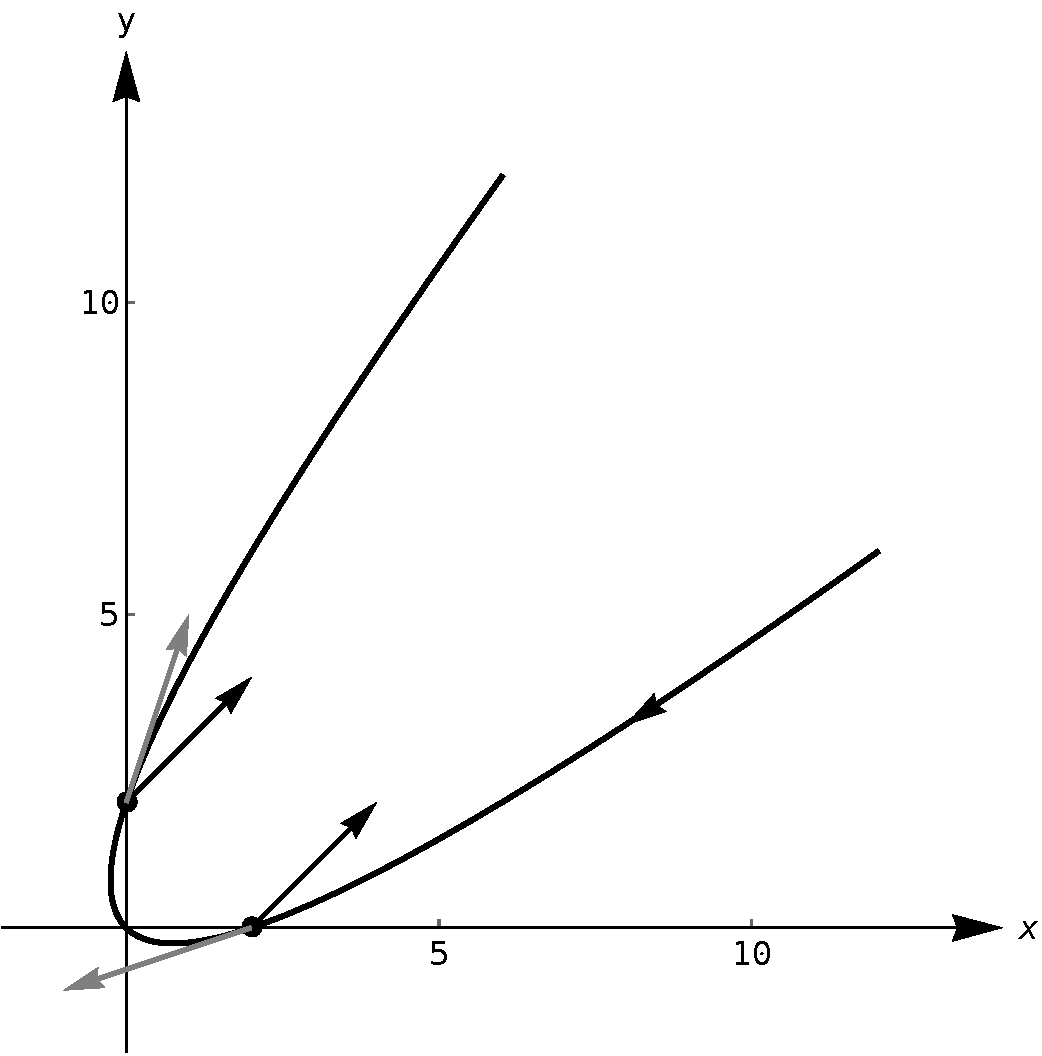
\includegraphics[width=0.43\textwidth]{fig_vector_fun_9a}}
\hspace{0.1cm}
\subfigure[\label{fig_vector_fun_9b}]{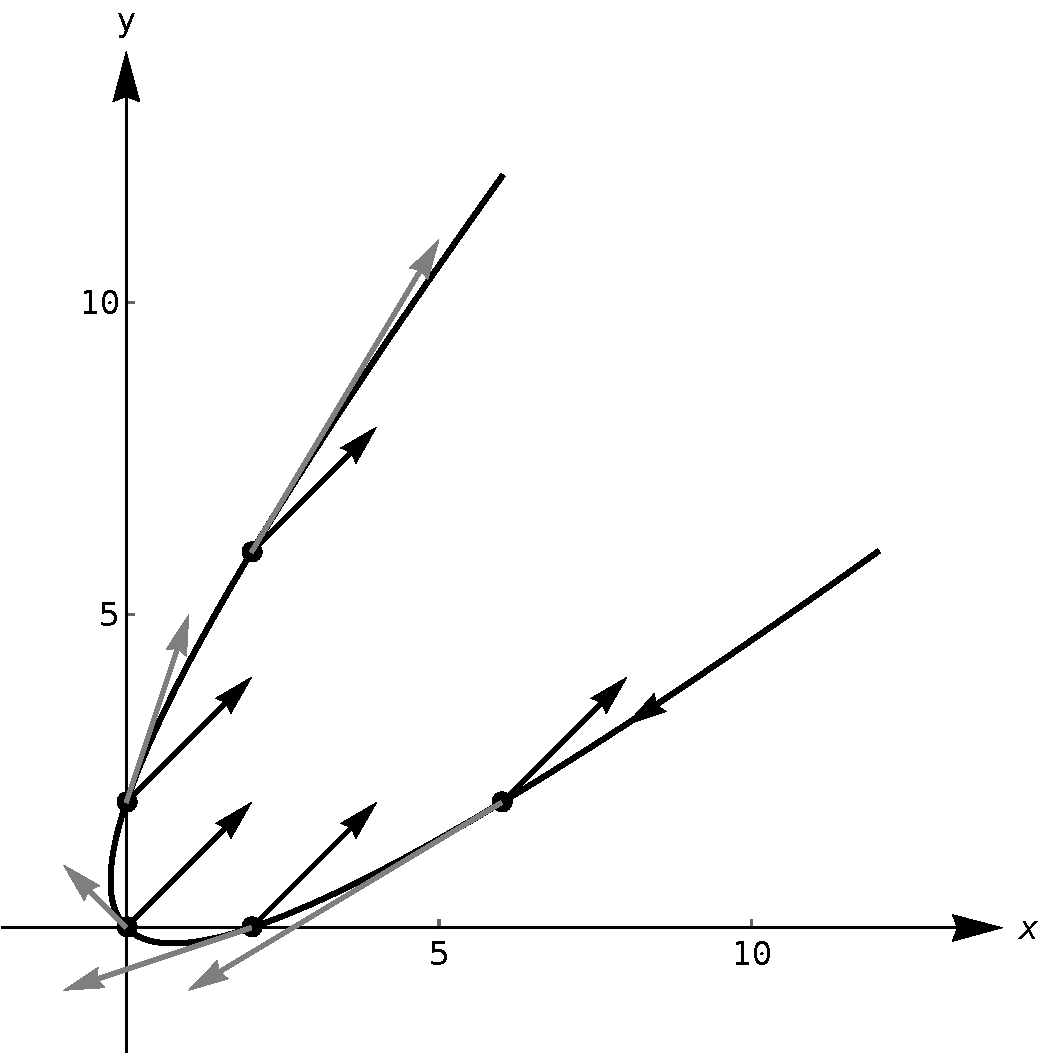
\includegraphics[width=0.43\textwidth]{fig_vector_fun_9b}}
}
\caption{Graphing the position (curve), velocity (gray) and acceleration (black) of an object in Example \ref{ex_motion1}.}
\end{figure}


\end{example}

If an object travels at a constant speed, we have $\norm{\vvt} = c$ for some constant $c$. Recall Theorem \ref{thm:vects_of_constant_length}, which states that if a vector--valued function \vrt\ has constant length, then \vrt\ is perpendicular to its derivative: $\vrt\cdot\vrp(t) = 0$. So, the corresponding velocity function has constant length, therefore we can conclude that the velocity is perpendicular to the acceleration: $\vvt\cdot\vat = 0$. 


An important application of vector--valued position functions is projectile motion: the motion of objects under only the influence of gravity. We will measure time in seconds, and distances will either be in meters or feet. We will show that we can completely describe the path of such an object knowing its initial position and initial velocity.

Suppose an object has initial position $\vec r(0) = \left( x_0,y_0\right)$ and initial velocity $\vec v(0) = \left( v_x,v_y\right)$. It is customary to rewrite $\vec v(0)$ in terms of its speed $v_0$ and direction $\vec u$, where $\vec u$ is a unit vector. Recall all unit vectors in $\mathbb{R}^2$ can be written as $\left( \cos (\theta),\sin (\theta)\right)$, where $\theta$ is an angle measure counter--clockwise from the $x$-axis. We refer to $\theta$ as the angle of elevation. Thus $\vec v(0) = v_0\left( \cos (\theta),\sin (\theta)\right).$ 

Since the acceleration of the object is known, namely $\vat = \left( 0,-g\right)$, where $g$ is the gravitational constant, we can find $\vrt$ knowing our two initial conditions. We first find $\vvt$:
\begin{align*}
\vec v(t) &= \int \vat \ dt\\
\Rightarrow \;  \vvt &= \int \left( 0,-g\right) \ dt\\
\Leftrightarrow \; \vvt &= \left( 0,-gt\right) + \vec C.
\end{align*}
Knowing $\vec v(0) = v_0\left( \cos(\theta),\sin(\theta)\right)$, we have $\vec C = v_0\left( \cos(\theta),\sin(\theta)\right)$ and so
$$\vec v(t) = \left(\rule{0pt}{9pt} v_0\cos(\theta), -gt+v_0\sin(\theta)\right).$$
We integrate once more to find $\vrt$:
\allowdisplaybreaks
\begin{align*}
\vrt &= \int \vvt\ dt \\
\vrt &= \int \left( \rule{0pt}{9pt} v_0\cos(\theta), -gt+v_0\sin(\theta)\right)\ dt\\
\vrt &= \left(  \big(v_0\cos(\theta)\big)t, -\frac12gt^2+\big(v_0\sin(\theta)\big)t\right) + \vec C.
\intertext{Knowing $\vec r(0) = \left( x_0,y_0\right)$, we conclude $\vec C = \left( x_0,y_0\right)$ and }
\vrt &= \left( \big(v_0\cos(\theta)\big)t+x_0\ , -\frac12gt^2+\big(v_0\sin(\theta)\big)t+y_0\ \right). %\\
%\vrt &= \left( 0,-\frac12g\right) t^2 + v_0\left( \cos\theta,\sin \theta\right) t + \left( x_0,y_0\right).
\end{align*}
This is the position function of a projectile propelled from an initial position of $\vec r_0=\left( x_0,y_0\right)$, with initial speed $v_0$, with angle of elevation $\theta$ and neglecting all accelerations but gravity.

We can also rely on vector--valued functions to compute the distance travelled. For instance, consider a driver who sets her cruise--control to 60 km/h, and travels at this speed for an hour. We can ask:
\begin{enumerate}
	\item How far did the driver travel?
	\item	How far from her starting position is the driver?
\end{enumerate} 
The first is easy to answer: she travelled 60 kilometres. The second is impossible to answer with the given information. We do not know if she travelled in a straight line, on an oval racetrack, or along a slowly--winding highway.

This highlights an important fact: to compute distance travelled, we need only to know the speed, given by $\norm{\vvt}$.

\begin{definition}[Distance travelled]\label{thm:distance_traveled}
Let $\vvt$ be a velocity function for a moving object. The \textbf{distance travelled} (\textit{afgelegde afstand}) by the object on $[a,b]$ is:
\index{distance!traveled}\index[aut]{afgelegde afstand}
$$\text{distance travelled} = \int\limits_a^b \norm{\vvt}\ dt.$$
\end{definition}
Note that this is just a restatement of Theorem \ref{thm:vvf_arc_length}: arc length is the same as distance travelled, just viewed in a different context.


\begin{example}\label{ex_motion6}
A particle moves in space with position function $\vrt = \left( t,t^2,\sin (\pi t)\right)$ on $[-2,2]$, where $t$ is measured in seconds and distances are in meters. Find:
\begin{enumerate}
	\item The distance travelled by the particle on $[-2,2]$.
	\item	The displacement of the particle on $[-2,2]$.
	\item	The particle's average speed.
\end{enumerate}

\xhrulefill{gray}{2.5pt}Solution \xhrulefill{gray}{2.5pt}

\begin{enumerate}
	\item We use Definition~\ref{thm:distance_traveled} to establish the integral:
	\begin{align*}
	\text{distance travelled} &= \int\limits_{-2}^2 \norm{\vvt}\ dt \\
							&= \int\limits_{-2}^2 \sqrt{1+(2t)^2+ \pi^2\cos^2(\pi t)}\ dt.
	\end{align*}
	This cannot be solved in terms of elementary functions so we turn to numerical integration, finding the distance to be 12.88m.
	
	\item		The displacement is the vector $$\vec r(2)-\vec r(-2) = \left( 2,4,0\right) - \left( -2,4,0\right) = \left( 4,0,0\right).$$ That is, the particle ends with an $x$-value increased by 4 and with $y$- and $z$-values the same.
	
	\item		We found above that the particle travelled 12.88m over 4 seconds. We can compute average speed by dividing: 12.88/4 = 3.22 m/s.
	We should also consider Definition \ref{def:av_val} to compute the average value of the speed as
	$$\text{average speed} = \frac{1}{2-(-2)}\int\limits_{-2}^2 \norm{\vvt}\ dt \approx \frac14 12.88 = 3.22\text{m/s}.$$

\end{enumerate}
\begin{figure}[H]
\centering
%\right)isebox{0.5cm}{
\centerline{
\subfigure[\label{fig_vector_fun_10a}]{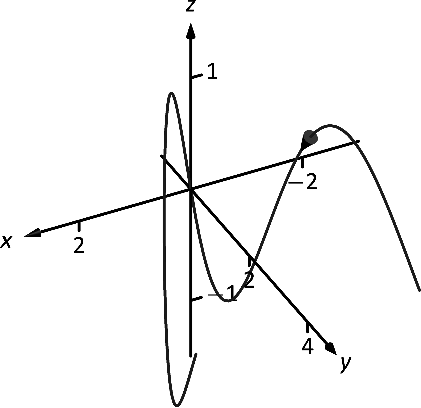
\includegraphics[width=0.3\textwidth]{fig_vector_fun_10a}}
\hspace{1cm}
\subfigure[\label{fig_vector_fun_10b}]{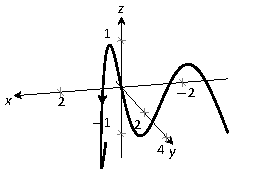
\includegraphics[width=0.44\textwidth]{fig_vector_fun_10b}}
}
\caption{The path of the particle, from two perspectives, in Example \ref{ex_motion6}.}
\end{figure}
\vspace*{-0.5cm}
\end{example}

Note how in Example \ref{ex_motion6} we computed the average speed as the average value of $\norm{\vvt}$ on $[-2,2]$.

Likewise, given the position function $\vrt$, the average velocity on $[a,b]$ is
$$\frac{\text{displacement}}{\text{travel time}} = \frac1{b-a}\int\limits_a^b \vec{r}\,'(t)\ dt = \frac{\vec r(b)-\vec r(a)}{b-a},$$
that is, it is the average value of $\vec r\,'(t)$, or $\vvt$, on $[a,b]$.\\

\section{Unit tangent and normal vectors}\label{sec:tan_norm}

Given a smooth vector--valued function \vrt, we defined in Definition \ref{def:vector_tangent} that any vector parallel to $\vrp(t_0)$ is tangent to the graph of \vrt\ at $t=t_0$. It is often useful to consider just the direction of $\vrp(t)$ and not its magnitude. Therefore we are interested in the unit vector in the direction of $\vrp(t)$. This leads to a definition.

\begin{definition}[Unit tangent vector]\label{def:unit_tangent}
Let \vrt\ be a smooth function on an open interval $I$. The \textbf{unit tangent vector $\widehat T(t)$} (\textit{eenheids\-raakvector}) is
\index{unit tangent vector!definition} \index{unit vector!unit tangent vector}
$$\widehat T(t) = \frac{1}{\rule{0pt}{9pt}\norm{\vrp(t)}}\vrp(t).$$
\end{definition}

Just as knowing the direction tangent to a path is important, knowing a direction orthogonal to a path is important. When dealing with real-valued functions, we defined the normal line at a point to be the line through the point that was perpendicular to the tangent line at that point. We can do a similar thing with vector--valued functions. Given \vrt\ in $\mathbb{R}^2$, we have 2 directions perpendicular to the tangent vector, as shown in Figure \ref{fig_vector_fun_11}. 


\begin{figure}[H]
	\begin{center}
			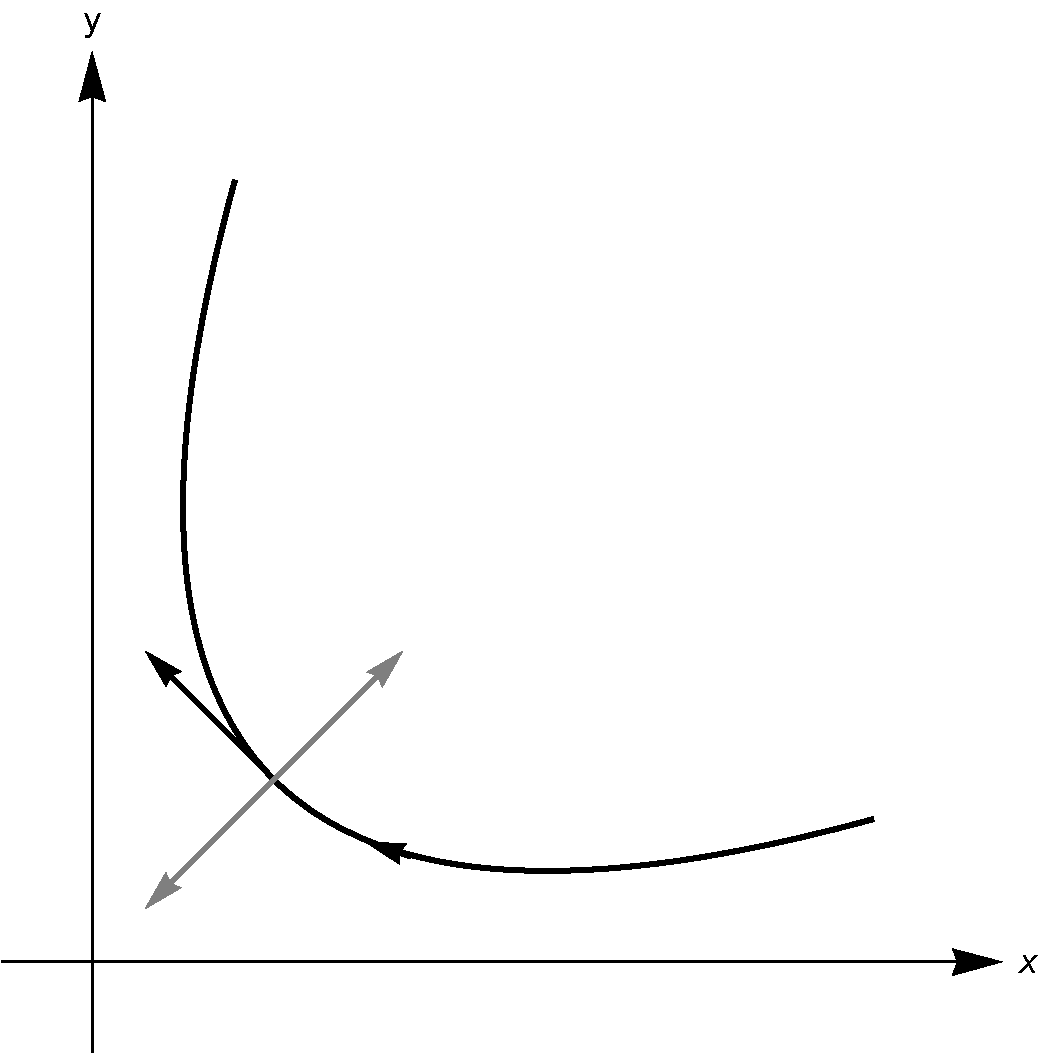
\includegraphics[width=0.4\textwidth]{fig_vector_fun_11}
	\caption{Given a direction in the plane, there are always two directions orthogonal to it.}
	\label{fig_vector_fun_11}
	\end{center}
\end{figure}


Given \vrt\ in $\mathbb{R}^3$,  there are infinitely many vectors orthogonal to the tangent vector at a given point. We might wonder whether one of these infinite choices preferable over the others.

The answer in both $\mathbb{R}^2$ and $\mathbb{R}^3$ is ``Yes, there is one vector that is not only preferable, it is the right one to choose. Recall that if \vrt\ has constant length, then \vrt\ is orthogonal to $\vrp(t)$ for all $t$. We know $\widehat T(t)$, the unit tangent vector, has constant length. Therefore $\widehat T(t)$ is orthogonal to $\widehat T\,'(t)$.

We will see that $\widehat T\,'(t)$ is more than just a convenient choice of vector that is orthogonal to $\vrp(t)$; rather, it is the right choice. Since all we care about is the direction, we define this newly found vector to be a unit vector. Note that if $\widehat T(t)$ is a unit vector, this does not imply that $\widehat T\,'(t)$ is also a unit vector.


\begin{definition}[Unit normal vector]\label{def:unit_normal}
Let \vrt\ be a vector--valued function where the unit tangent vector, $\widehat T(t)$, is smooth on an open interval $I$. The \textbf{unit normal vector $\widehat N(t)$} (\textit{eenheidsnormaalvector}) is
\index{unit normal vector!definition}\index{unit vector!unit normal vector}
$$\widehat N(t) = \frac1{\norm{\widehat T\,'(t)}}\widehat T\,'(t).$$
\end{definition}



\begin{example}\label{ex_tannorm2}
Let $$\vrt=\left( t^2-t,t^2+t\right).$$
\begin{enumerate}
\item Find $\widehat T(t)$ and compute $\widehat T(0)$ and $\widehat T(1)$.
\item Find $\widehat N(t)$ and sketch $\vrt$ with the unit tangent and normal vectors at $t=-1,0$ and 1.
\end{enumerate}

\xhrulefill{gray}{2.5pt}Solution \xhrulefill{gray}{2.5pt}

\begin{enumerate}
\item We find $\vrp(t) = \left( 2t-1,2t+1\right)$, and $$\norm{\vrp(t)} = \sqrt{(2t-1)^2+(2t+1)^2} = \sqrt{8t^2+2}.$$
Therefore $$\widehat T(t) =\frac{1}{\rule{0pt}{9pt}\norm{\vrp(t)}}\vrp(t)= \frac{1}{\sqrt{8t^2+2}}\left( 2t-1,2t+1\right) = \left( \frac{2t-1}{\sqrt{8t^2+2}},\frac{2t+1}{\sqrt{8t^2+2}}\right).$$
When $t=0$, we have $\widehat T(0) = \left( -1/\sqrt{2},1/\sqrt{2}\right)$; when $t=1$, we have $\widehat T(1) = \left( 1/\sqrt{10}, 3/\sqrt{10}\right).$ We leave it to the reader to verify each of these is a unit vector. 
\item Given $\widehat T(t)$, finding $\widehat T\,'(t)$ requires two applications of the quotient rule:

\begin{align*}
T\,'(t) &= \left( \frac{\sqrt{8t^2+2}(2)-(2t-1)\left(\frac12(8t^2+2)^{-1/2}(16t)\right)}{8t^2+2},\right.\\
		&\phantom{xxxxxxxxx} \left.\frac{\sqrt{8t^2+2}(2)-(2t+1)\left(\frac12(8t^2+2)^{-1/2}(16t)\right)}{8t^2+2} \right) \\[0.2cm]
				&= \left( \frac{4 (2 t+1)}{\left(8 t^2+2\right)^{3/2}},\frac{4
   (1-2 t)}{\left(8 t^2+2\right)^{3/2}}\right).
\end{align*}

This is not a unit vector; to find $\widehat N(t)$, we need to divide $\widehat T\,'(t)$ by its magnitude:
\allowdisplaybreaks
\begin{align*}
\norm{\widehat T\,'(t)} &= \sqrt{\frac{16(2t+1)^2}{(8t^2+2)^3}+\frac{16(1-2t)^2}{(8t^2+2)^3}}\\[0.2cm]
					&= \sqrt{\frac{16(8t^2+2)}{(8t^2+2)^3}}\\[0.2cm]
					&= \frac{4}{8t^2+2}.
\end{align*}
Finally, 
\begin{align*}
\widehat N(t) =\frac{1}{\rule{0pt}{9pt}\norm{\widehat T'(t)}}\widehat T'(t)&= \frac1{4/(8t^2+2)}\left( \frac{4 (2 t+1)}{\left(8 t^2+2\right)^{3/2}},\frac{4
   (1-2 t)}{\left(8 t^2+2\right)^{3/2}}\right)\\[0.2cm]
	&= \left( \frac{2t+1}{\sqrt{8t^2+2}},-\frac{2t-1}{\sqrt{8t^2+2}}\right).
\end{align*}

Using this formula for $\widehat N(t)$, we compute the unit tangent and normal vectors for $t=-1,0$ and 1 and sketch them in Figure \ref{fig_vector_fun_12}.

\end{enumerate}

\begin{figure}[H]
	\begin{center}
			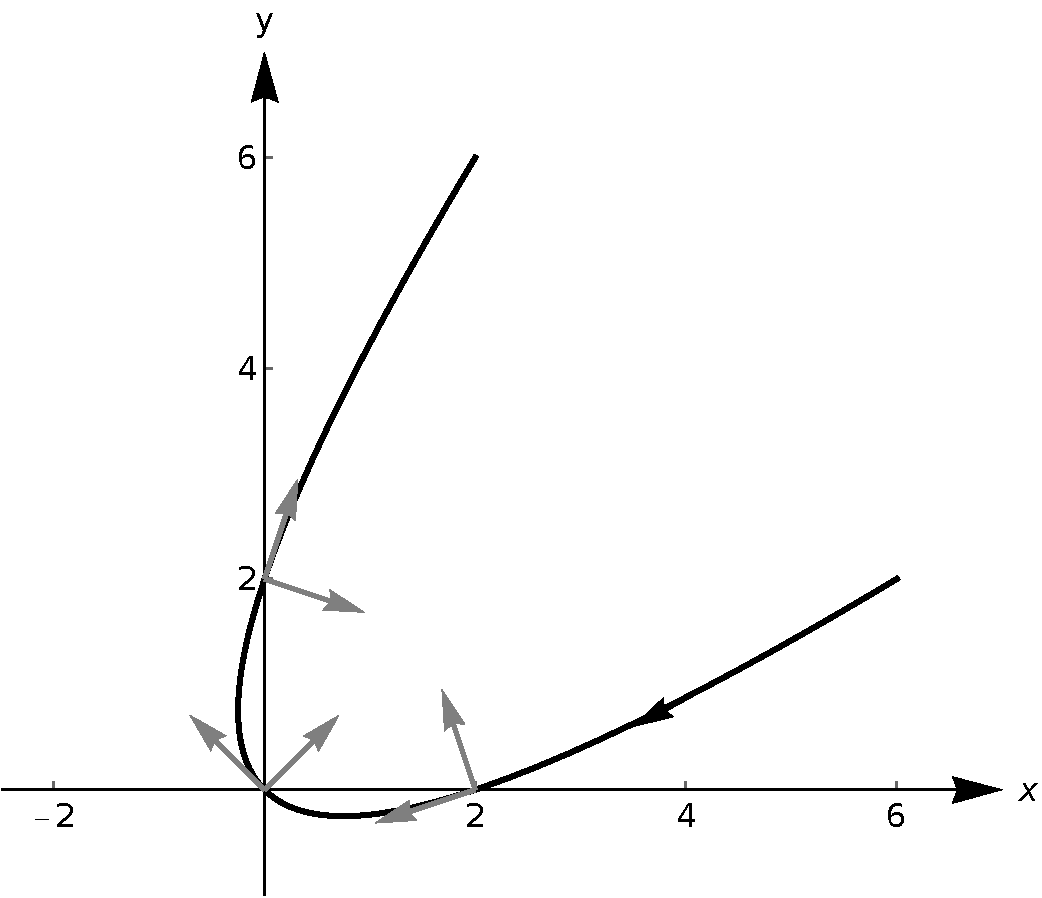
\includegraphics[width=0.45\textwidth]{fig_vector_fun_12}
	\caption{Unit tangent and normal vectors from Example \ref{ex_tannorm2}.}
	\label{fig_vector_fun_12}
	\end{center}
\end{figure}


\end{example}

The final 	result for $\widehat N(t)$ in Example \ref{ex_tannorm2} is suspiciously similar to $\widehat T(t)$. There is a clear reason for this. If $\vec u = \left( u_1,u_2\right) $ is a unit vector in $\mathbb{R}^2$, then the only unit vectors orthogonal to $\vec u$ are $\left( -u_2,u_1\right) $ and $\left( u_2,-u_1\right)$. Given $\widehat T(t)$, we can quickly determine $\widehat N(t)$ if we know which term to multiply by $(-1)$.
Consider again Figure \ref{fig_vector_fun_12}, where we have plotted some unit tangent and normal vectors. Note how $\widehat N(t)$ always points inside the curve, or to the concave side of the curve. This is not a coincidence; this is true in general. Knowing the direction that $\vec r(t)$ turns allows us to quickly find $\widehat N(t)$.


\begin{theorem}[Unit normal vectors in $\mathbb{R}^2$]\label{thm:concave}
Let $\vec r(t)$ be a vector--valued function in $\mathbb{R}^2$ where $\widehat T\,'(t)$ is smooth on an open interval $I$. Let $t_0$ be in $I$ and $\widehat T(t_0) = \left( t_1,t_2\right)$ Then $\widehat N(t_0)$ is either
$$\widehat N(t_0) = \left( -t_2,t_1\right) \quad \text{or}\quad \widehat N(t_0) = \left( t_2,-t_1\right),$$ whichever is the vector that points to the concave side of the graph of $\vec r$.
\end{theorem}


\section{Arc length and curvature}\label{sec:curvature}
\subsection{Arc length}
Currently, our vector--valued functions have defined points with a parameter $t$, which we often take to represent time. Consider Figure \ref{fig_vector_fun_13a}, where $\vrt = \left( t^2-t,t^2+t\right)$ is graphed and the points corresponding to $t=0,\ 1$ and $2$ are shown. Note how the arc length between $t=0$ and $t=1$ is smaller than the arc length between $t=1$ and $t=2$; if the parameter $t$ is time and $\vec r$ is position, we can say that the particle travelled faster on $[1,2]$ than on $[0,1]$. 

Now consider Figure \ref{fig_vector_fun_13b}, where the same graph is parametrized by a different variable $s$.  Points corresponding to $s=0$ through $s=6$ are plotted. The arc length of the graph between each adjacent pair of points is 1. We can view this parameter $s$ as distance; that is, the arc length of the graph from $s=0$ to $s=3$ is 3, the arc length from $s=2$ to $s=6$ is 4, etc. If one wants to find the point 2.5 units from an initial location (i.e., $s=0$), one would compute $\vec r(2.5)$. This parameter $s$ is very useful, and is called the \textbf{arc length parameter}.\index{arc length parameter}\index{arc length}\index[aut]{booglengte}


\begin{figure}[H]
\centering
%\right)isebox{0.5cm}{
\centerline{
\subfigure[\label{fig_vector_fun_13a}]{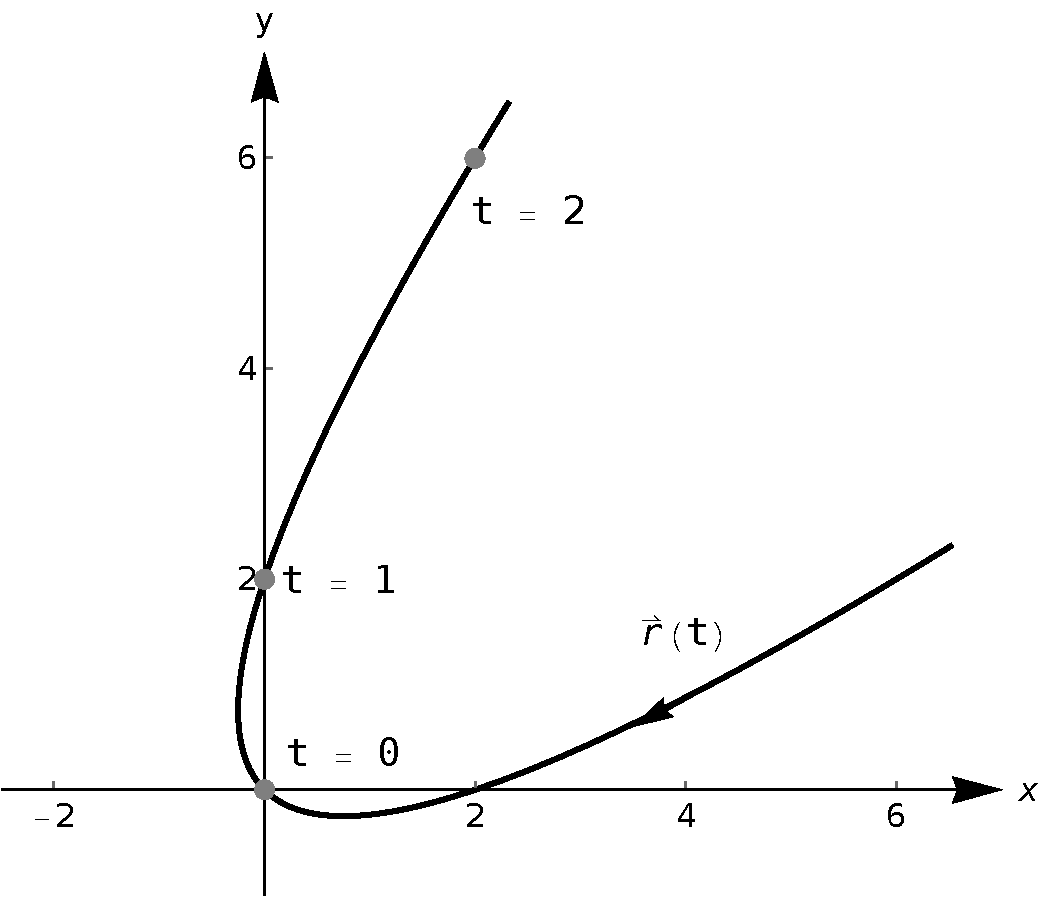
\includegraphics[width=0.43\textwidth]{fig_vector_fun_13a}}
\hspace{0.1cm}
\subfigure[\label{fig_vector_fun_13b}]{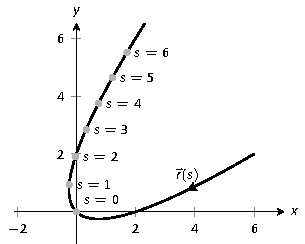
\includegraphics[width=0.43\textwidth]{fig_vector_fun_13b}}
}
\caption{Introducing the arc length parameter.}
\end{figure}


How do we find the arc length parameter? 


Start with any parametrization of $\vec r$. We can compute the arc length of the graph of $\vec r$ on the interval $[0,t]$ with 
$$\text{arc length } = \int\limits_0^t\norm{\vec r\,'(u)}\ du.$$
 We can turn this into a function: as $t$ varies, we find the arc length $s$ from $0$ to $t$. This function is
\begin{equation}
s(t) = \int\limits_0^t \norm{\vec r\,'(u)}\ du.\label{eq:vvfarc}
\end{equation}

This establishes a relationship between $s$ and $t$. Knowing this relationship explicitly, we can rewrite $\vec r(t)$ as a function of $s$: $\vec r(s)$. We demonstrate this in an example.




\begin{example}\label{ex_vvfarc1}
Let $\vec r(t) = \left( 3t-1,4t+2\right)$. Parametrize $\vec r$ with the arc length parameter $s$.

\xhrulefill{gray}{2.5pt}Solution \xhrulefill{gray}{2.5pt}

Using Equation \eqref{eq:vvfarc}, we write
$$s(t) = \int\limits_0^t \norm{\vec r\,'(u)}\ du.$$
We can integrate this, explicitly finding a relationship between $s$ and $t$:
\allowdisplaybreaks
\begin{align*}
s(t) &= \int\limits_0^t \norm{\vec r\,'(u)}\ du \\[0.2cm]
			&= \int\limits_0^t \sqrt{3^2+4^2}\ du\\[0.2cm]
			&= \int\limits_0^t 5\ du\\[0.2cm]
			&= 5t.
\end{align*}
Since $s=5t$, we can write $t=s/5$ and replace $t$ in $\vec r(t)$ with $s/5$:
$$\vec r(s) = \left( 3\left(\dfrac{s}{5}\right)-1, 4\left(\dfrac{s}{5}\right)+2\right) = \left( \frac35s-1,\frac45s+2\right).$$
Clearly, as shown in Figure \ref{fig_vector_fun_14}, the graph of $\vec r$ is a line, where $t=0$ corresponds to the point $(-1,2)$. What point on the line is 2 units away from this initial point? We find it with \\ $\vec r(2) = \left( 1/5, 18/5\right)$. 


Is the point $(1/5,18/5)$ really 2 units away from $(-1,2)$? We use the distance formula to check:
$$d = \sqrt{\left(\frac15-(-1)\right)^2+ \left(\frac{18}5-2\right)^2} = \sqrt{\frac{36}{25}+\frac{64}{25}} = \sqrt{4}=2.$$
Yes, $\vec r(2)$ is indeed 2 units away, in the direction of travel, from the initial point.

\begin{figure}[H]
	\begin{center}
			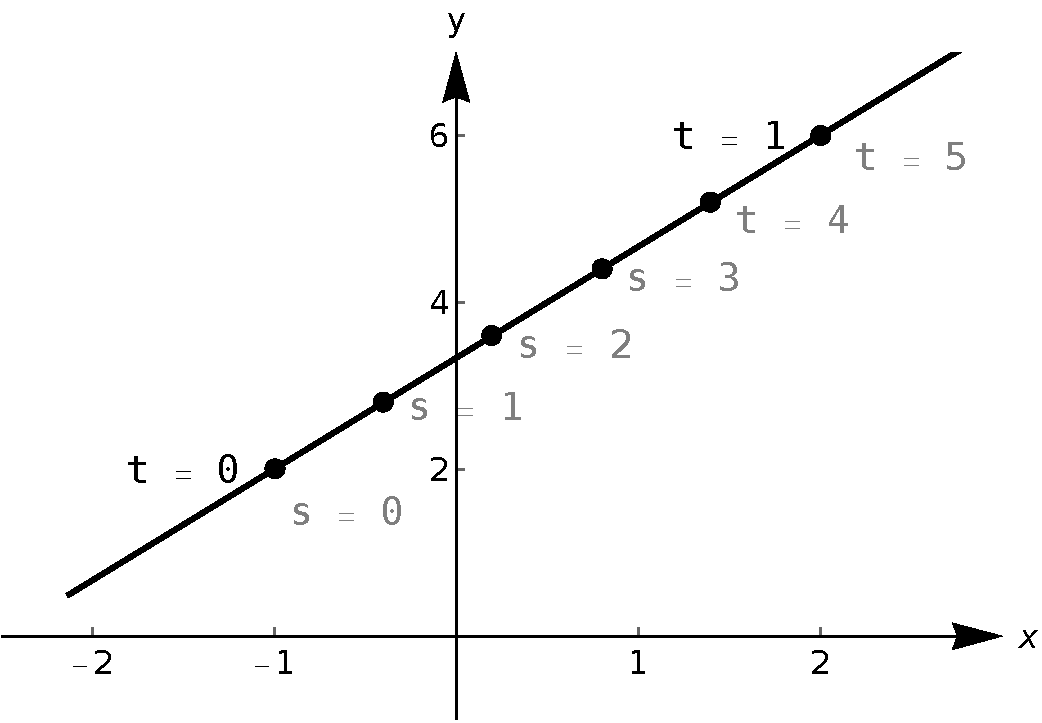
\includegraphics[width=0.4\textwidth]{fig_vector_fun_14}
	\caption{Graphing $\vec r$ in Example \ref{ex_vvfarc1} with parameters $t$ and $s$.}
	\label{fig_vector_fun_14}
	\end{center}
\end{figure}

\end{example}


Things worked out very nicely in Example \ref{ex_vvfarc1}; we were able to establish directly that $s=5t$. Usually, the arc length parameter is much more difficult to describe in terms of $t$, a result of integrating a square--root. There are a number of things that we can learn about the arc length parameter from Equation \eqref{eq:vvfarc}, though, that are useful.

First, %consider Equation \eqref{eq:vvfarc} and 
take the derivative of $s$ with respect to $t$. The fundamental theorem of calculus (see Theorem \ref{thm:FTC1}) states that
\begin{equation}
\frac{ds}{dt}=s\,'(t) = \norm{\vrp(t)}.\label{eq:vvfarc3}
\end{equation}
Letting $t$ represent time and $\vec r(t)$ represent position, we see that the rate of change of $s$ with respect to $t$ is speed; that is, the rate of change of distance travelled is speed, which should match our intuition.

The chain rule states that 
\begin{align*}
\frac{d\vec r}{dt} &= \frac{d\vec r}{ds}\frac{ds}{dt}\\
\vrp(t) &= \vrp(s) \norm{\vrp(t)}.
\end{align*}
Solving for $\vrp(s)$, we have 
\begin{equation}
\vrp(s) = \frac{\vrp(t)}{\norm{\vrp(t)}} = \widehat T(t),\label{eq:vvfarc2}
\end{equation}
where $\widehat T(t)$ is the unit tangent vector. Equation \eqref{eq:vvfarc2} is often misinterpreted, as one is tempted to think it states $\vrp(t) = \widehat T(t)$, but there is a big difference between $\vrp(s)$ and $\vrp(t)$. The key to take from it is that $\vrp(s)$ is a unit vector. In fact, the following definition states that this characterizes the arc length parameter.
	\checkoddpage
\marginpar{\ifoddpage\hspace*{-1.5cm}\else\hspace*{0.25cm}\fi
\includegraphics[width=0.075\textwidth]{youtube}\\
\ifoddpage\hspace*{-1.75cm}\else\hspace*{0.1cm}\fi
\qrcode[height=1.75cm]{https://youtu.be/S_WZdwglDWI}
%\includegraphics[width=0.1\textwidth]{arc_length_parameter}
}

\begin{definition}[Arc length parameter]\label{thm:arclengthparam}
Let $\vec r(s)$ be a vector--valued function. The parameter $s$ is the \textbf{arc length parameter} if, and only if, $\norm{\vrp(s)} = 1.$\index{arc length parameter}
\end{definition}

\subsection{Curvature}
Consider points $A$ and $B$ on the curve graphed in Figure \ref{fig_vector_fun_15a}. One can readily argue that the curve curves more sharply at $A$ than at $B$. It is useful to use a number to describe how sharply the curve bends; that number is the \textbf{curvature} (\textit{kromming}) of the curve.

\begin{figure}[H]
\centering
%\right)isebox{0.5cm}{
\centerline{
\subfigure[\label{fig_vector_fun_15a}]{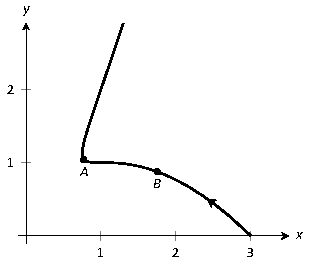
\includegraphics[width=0.4\textwidth]{fig_vector_fun_15a}}
\hspace{0.1cm}
\subfigure[\label{fig_vector_fun_15b}]{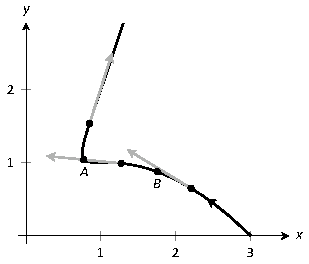
\includegraphics[width=0.4\textwidth]{fig_vector_fun_15b}}
}
\label{fig_vector_fun_15bis}
\caption{Establishing the concept of curvature.}
\end{figure}


We derive this number in the following way. Consider Figure \ref{fig_vector_fun_15b}, where  unit tangent vectors are graphed around points $A$ and $B$. Notice how the direction of the unit tangent vector changes quite a bit near $A$, whereas it does not change as much around $B$. This leads to an important concept: measuring the rate of change of the unit tangent vector with respect to arc length gives us a measurement of curvature.





\begin{definition}[Curvature]\label{def:curvature}
Let $\vec r(s)$ be a vector--valued function where $s$ is the arc length parameter. The \textbf{curvature $\kappa$} of the graph of $\vec r(s)$ is
\index{curvature}\index[aut]{kromming}
$$\kappa(t) = \snorm{\frac{d\widehat T}{ds}} = \snorm{\widehat T\,'(s)}.$$
\end{definition}



	\checkoddpage
\marginpar{\ifoddpage\hspace*{-1.5cm}\else\hspace*{0.25cm}\fi
\includegraphics[width=0.075\textwidth]{youtube}\\
\ifoddpage\hspace*{-1.75cm}\else\hspace*{0.1cm}\fi
\qrcode[height=1.75cm]{https://youtu.be/gspjhwSNMWs}
%\includegraphics[width=0.1\textwidth]{curvature}
}
If $\vec r(s)$ is parametrized by the arc length parameter, then 
$$\widehat T(s) = \frac{\vrp(s)}{\norm{\vrp(s)}} \quad \text{and}\quad \widehat N(s) = \frac{\widehat T\,'(s)}{\norm{\widehat T\,'(s)}}.$$
Having defined $\norm{\widehat T\,'(s)} =\kappa$, we can rewrite the second equation as
\begin{equation}\widehat T\,'(s) = \kappa\widehat N(s).\label{eq:curvature}
\end{equation}
We already knew that $\widehat T\,'(s)$ is in the same direction as $\widehat N(s)$; that is, we can think of $\widehat T(s)$ as being pulled in the direction of $\widehat N(s)$. How hard is it being pulled? By a factor of $\kappa$. When the curvature is large, $\widehat T(s)$ is being pulled hard and the direction of $\widehat T(s)$ changes rapidly. When $\kappa$ is small, $T(s)$ is not being pulled hard and hence its direction is not changing rapidly. 



\begin{example}\label{ex_curvature1}
Find the curvature of $\vrt = \left( 3t-1,4t+2\right)$.

\xhrulefill{gray}{2.5pt}Solution \xhrulefill{gray}{2.5pt}


In Example \ref{ex_vvfarc1}, we found that the arc length parameter was defined by $s=5t$, so \linebreak $\vec r(s) =\left( 3s/5-1, 4s/5+2\right)$ parametrized $\vec r$ with the arc length parameter. To find $\kappa$, we need to find $\widehat T\,'(s)$. 
\begin{align*}
\widehat T(s) &= \vrp(s)\qquad \text{(recall this is a unit vector)}\\
				&= \left( \dfrac{3}{5},\dfrac{4}{5}\right).
\intertext{Therefore}
\widehat T\,'(s) &= \left( 0,0\right)
\intertext{and}
\kappa&=\snorm{\widehat T\,'(s)} = 0.
\end{align*}
It probably comes as no surprise that the curvature of a line is 0.
\end{example}


While the definition of curvature is a beautiful mathematical concept, it is nearly impossible to use most of the time; writing $\vec r$ in terms of the arc length parameter is generally very hard. Fortunately, there are other methods of calculating this value that are much easier. \ifcalculus There is a trade-off: the definition is easy to understand though hard to compute, whereas these other formulas are easy to compute though it may be hard to understand why they work.\fi

\ifanalysis\pagebreak\fi
\begin{theorem}[Formulas for curvature]\label{thm:curvature_formulas}
Let $C$ be a smooth curve  in the plane or in space.
\index{curvature!equations for}
\begin{enumerate}
	\item If $C$ is defined in space by a vector--valued function $\vec r(t)$, then
$$\kappa(t) = \frac{\norm{\widehat T\,'(t)}}{\norm{\vrp(t)}} = \frac{\norm{\vrp(t)\times\vrp'(t)}}{\norm{\vrp(t)}^3} = \frac{\vec a(t)\cdot \widehat N(t)}{\norm{\vec v(t)}^2}.$$
	\item If $C$ is defined by $y=f(x)$, then 
	$$\kappa = \frac{|\fp'(x)|}{\Big(1+\big(\fp(x)\big)^2\Big)^{3/2}}.$$
	\item	If $C$ is defined as a vector--valued function in the plane, $\vec r(t) = \left( x(t), y(t)\right)$, then
	$$\kappa = \frac{|x'y''-x''y'|}{\big((x')^2+(y')^2\big)^{3/2}}.$$
\end{enumerate}
\end{theorem}

\ifanalysis

\begin{proof}


To show the first statement in this theorem, we resort to the chain rule, i.e.
$$
\frac{d\widehat T}{dt} = \frac{d\widehat T}{ds}\frac{ds}{dt}= \frac{d\widehat T}{ds}\norm{\vrp(t)}\,,
$$
or after rearranging
$$
\frac{d\widehat T}{ds}=\dfrac{\frac{d\widehat T}{dt}}{\norm{\vrp(t)}}=\frac{\widehat T'(t)}{\norm{\vrp(t)}}\,.
$$
Consequently, we find that
$$
\kappa(t)=\norm{\dfrac{d\widehat{T}}{ds}}=\frac{\norm{\widehat T'(t)}}{\norm{\vrp(t)}}\,.
$$
Subsequently, we can show that
$$
\kappa(t) = \frac{\norm{\vrp(t)\times\vrp'(t)}}{\norm{\vrp(t)}^3} 
$$
by expressing $\vrp(t)$ and $\vrp'(t)$ in terms of $\widehat{T}$ and $\widehat{T}'$ and subsequently compute their cross product. For what concerns $\vrp(t)$, we recall that $\frac{ds}{dt}=\norm{\vrp(t)}$ and $ \widehat T(t) \frac{\vrp(t)}{\norm{\vrp(t)}}$, so we infer

$$\vrp(t)=\frac{ds}{dt}\widehat{T}\,.$$
Computing the derivative of this expression with respect to $t$ yields
$$
\vrp'(t)=\frac{d^2s}{dt^2}\widehat{T}+\frac{ds}{dt}\widehat{T}'\, 
$$
so that the cross product $\vrp(t)\times\vrp'(t)$ becomes
$$
\vrp(t)\times\vrp'(t)=\frac{ds}{dt}\frac{d^2s}{dt^2}\left(\widehat{T}\times\widehat{T}\right)+\left(\frac{ds}{dt}\right)^2\left(\widehat{T}\times\widehat{T}'\right)\,.
$$
Since the cross product of a vector by itself is always the zero vector,we see that
\begin{eqnarray*}
\norm{\vrp(t)\times\vrp'(t)}&=&\left(\frac{ds}{dt}\right)^2\left\|\widehat{T}\times\widehat{T}'\right\|\\[0.2cm]
&=&\left(\frac{ds}{dt}\right)^2\norm{\widehat{T}}\norm{\widehat{T}'}\sin(\theta)\,,
\end{eqnarray*}
where $\theta$ is the angle between $\widehat{T}$ and $\widehat{T}'$. Since $\norm{\widehat{T}}=1$ as a consequence of Equation~\eqref{eq:vvfarc2} and Definition~\ref{thm:arclengthparam}, and $\widehat{T}$ and $\widehat{T}'$ are perpendicular, we get that 
$$
\norm{\vrp(t)\times\vrp'(t)}=\left(\frac{ds}{dt}\right)^2\norm{\widehat{T}'}=\norm{\vec{r}'(t)}^2\norm{\widehat{T}'}\,.
$$
Therefore,
$$
\norm{\widehat{T}'}=\dfrac{\norm{\vrp(t)\times\vrp'(t)}}{\norm{\vec{r}'(t)}^2}\,
$$
and
\begin{equation}
\kappa(t)=\frac{\norm{\widehat T'}}{\norm{\vrp(t)}}=\dfrac{\norm{\vrp(t)\times\vrp'(t)}}{\norm{\vec{r}'(t)}^3}\,.
\label{kappa3}
\end{equation}
The proof of the second statement in the theorem follows easily from Equation~\eqref{kappa3} after acknowledging that it is easy to parameterise the curve given by $y=f(x)$ as a 3D parametric curve. Indeed, 
we can simply use $x=x$, $y=f(x)$ and $z=0$, where $x$ is considered a parameter. 

Starting from Equation~\eqref{kappa3} and letting $\vec r(t) = \left( x(t), y(t)\right)$ we easily get the third statement in the theorem. 
%link met verandering hoek raaklijn: http://web.cs.iastate.edu/~cs577/handouts/curvature.pdf
%afleiden 1 en 3: http://ksuweb.kennesaw.edu/~plaval/math2203/curvature.pdf
%afleiden 2: http://www-users.math.umn.edu/~mille003/1372curvature.pdf
%Of OpenStax: https://cnx.org/contents/oxzXkyFi@3.1:9fEOYsBF@8/Arc-Length-and-Curvature
\end{proof}

\fi

\begin{example}\label{ex_curvature2}
Find the curvature of a circle with radius $r$, defined by $\vec c(t) = \left( r\cos(t),r\sin(t)\right)$.

\xhrulefill{gray}{2.5pt}Solution \xhrulefill{gray}{2.5pt}

Before we start, we should expect the curvature of a circle to be constant, and not dependent on $t$. 

We compute $\kappa$ using the second part of Theorem \ref{thm:curvature_formulas}:
\begin{align*}
\kappa &= \frac{\Big|\big(-r\sin(t)\big)\big(-r\sin(t)\big) - \big(-r\cos(t)\big)\big(r\cos(t)\big)\Big|}{\Big( \big(-r\sin (t))^2+(r\cos(t)\big)^2\Big)^{3/2}} \\[0.2cm]
			&= \rule{0pt}{20pt}\frac{r^2\big(\sin^2(t)+\cos^2(t)\big)}{\Big(r^2\big(\sin^2(t)+\cos^2(t)\big)\Big)^{3/2}}\\[0.2cm]
			&= \rule{0pt}{20pt}\frac{r^2}{r^3} = \frac1r.
\end{align*}
We have found that a circle with radius $r$ has curvature $\kappa = 1/r$.
\end{example}

Example \ref{ex_curvature2} gives a great result. Before this example, if we were told ``The curve has a curvature of 5 at point $A$,'' we would have no idea what this really meant. Is 5 big -- does is correspond to a really sharp turn, or a not-so-sharp turn? Now we can think of 5 in terms of a circle with radius 1/5. Knowing the units  allows us to determine how sharply the curve is curving.


Let a point $P$ on a smooth curve $C$  be given, and let $\kappa$ be the curvature of the curve at $P$. A circle that:
	\begin{itemize}
		\item passes through $P$,
		\item	lies on the concave side of $C$,
		\item	has a common tangent line as $C$ at $P$, and
		\item	has radius $r=1/\kappa$ (hence has curvature $\kappa$)
	\end{itemize}
	
is the \textbf{osculating circle} (\textit{osculatiecirkel}), or \textbf{circle of curvature}, to $C$ at $P$, and $r$ is the \textbf{radius of curvature} (\textit{kromtestraal}). \index[aut]{kromtestraal}\index{osculating circle}\index{circle of curvature}\index{radius of curvature}\index[aut]{osculatiecirkel}%
Figure \ref{fig_vector_fun_16} shows the graph of the curve seen earlier in Figure \ref{fig_vector_fun_15a} and its osculating circles at $A$ and $B$. A sharp turn corresponds to a circle with a small radius; a gradual turn corresponds to a circle with a large radius. Being able to think of curvature in terms of the radius of a circle is very useful. The word osculating comes from a Latin word related to kissing; an osculating circle kisses the graph at a particular point. Many beautiful ideas in mathematics have come from studying the osculating circles to a curve. 


\begin{figure}[h]
	\begin{center}
			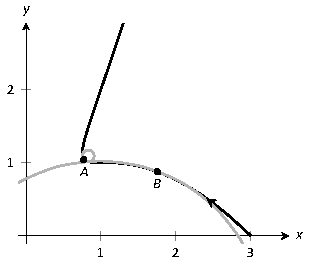
\includegraphics[width=0.45\textwidth]{fig_vector_fun_16}
	\caption{Illustrating the osculating circles for the curve seen in Figure \ref{fig_vector_fun_15a}.}
	\label{fig_vector_fun_16}
	\end{center}
\end{figure}

\begin{example}\label{ex_curvature4}
Find where the curvature of $\vec r(t) = \left( t, t^2, 2t^3\right) $ is maximized.

\xhrulefill{gray}{2.5pt}Solution \xhrulefill{gray}{2.5pt}

We use the third formula in Theorem \ref{thm:curvature_formulas} as $\vrt$ is defined in space. We leave it to the reader to verify that 
$$\vrp(t) =\left( 1,2t,6t^2\right),\quad \vrp'(t) = \left( 0,2,12t\right),\quad \text{and}\quad \vrp(t)\times \vrp'(t) = \left( 12t^2,-12t,2\right).$$

Thus 
\allowdisplaybreaks
\begin{align*}
\kappa(t) &= \frac{\norm{\vrp(t)\times\vrp'(t)}}{\norm{\vrp(t)}^3} \\[0.2cm]
				&= \rule{0pt}{20pt}\frac{\norm{\left( 12t^2,-12t,2\right)}}{\norm{\left( 1,2t,6t^2\right)}^3} \\[0.2cm]
				&= \rule{0pt}{20pt}\frac{\sqrt{\rule{0pt}{8.5pt}144t^4+144t^2+4}}{\left(\sqrt{\rule{0pt}{8.5pt}1+4t^2+36t^4\ }\right)^3}.\\[0.2cm]
\end{align*}
While this is not a particularly nice formula, it does explicitly tell us what the curvature is at a given $t$ value. To maximize $\kappa(t)$, we should solve $\kappa'(t)=0$ for $t$. This is doable, but  time consuming. Instead, consider the graph of $\kappa(t)$ as given in Figure \ref{fig_vector_fun_17a}. We see that $\kappa$ is maximized at two $t$ values; using a numerical solver, we find these values are $t\approx\pm 0.189$. In Figure~\ref{fig_vector_fun_17b} we graph $\vrt$ and indicate the points where curvature is maximized.

\begin{figure}[H]
\centering
%\right)isebox{0.5cm}{
\centerline{
\subfigure[\label{fig_vector_fun_17a}]{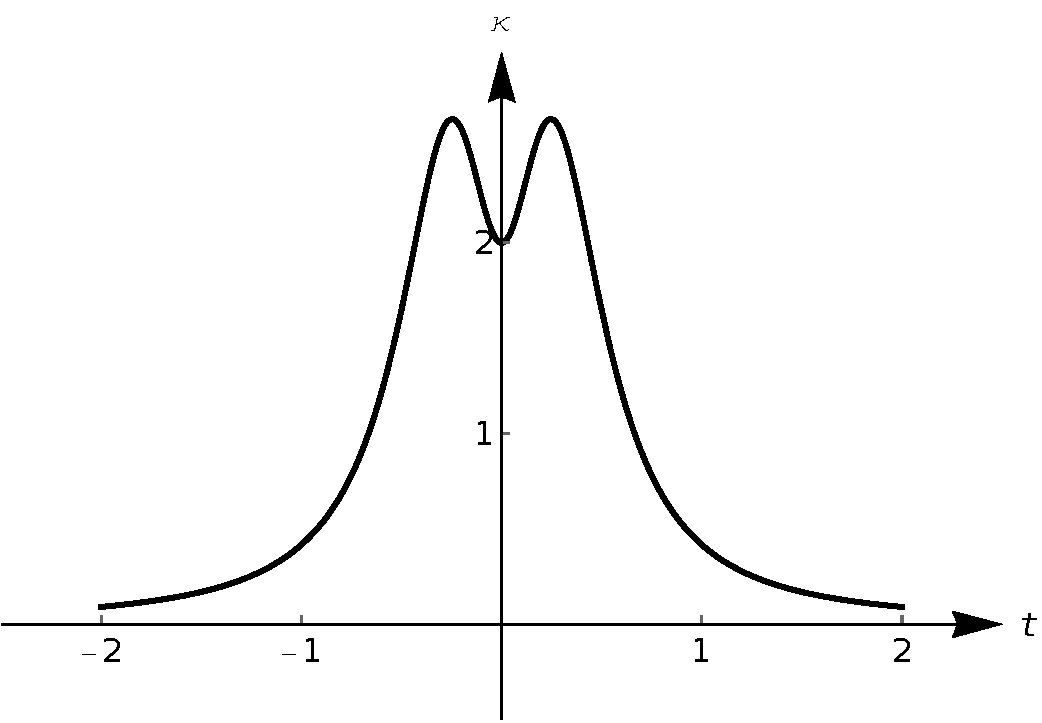
\includegraphics[width=0.43\textwidth]{fig_vector_fun_17a}}
\hspace{0.1cm}
\subfigure[\label{fig_vector_fun_17b}]{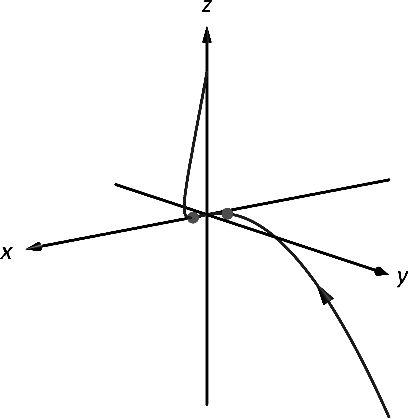
\includegraphics[width=0.33\textwidth]{fig_vector_fun_17b}}
}
\caption{Understanding the curvature of a curve in space.}
\end{figure}

\end{example}


We started this chapter with vector--valued functions, which may have seemed at the time to be just another way of writing parametric equations. However, we have seen that the vector perspective has given us great insight into the behaviour of functions and the study of motion. Vector--valued position functions convey displacement, distance travelled, speed, velocity, acceleration and curvature information, each of which has great importance in science and engineering.


\newpage
\section{Exercices}
\renewcommand{\ExerciseListName}{Assignement}

\subsection*{\nameref{subsec:alg_vect}}
%%%%%%%%%%%%%%%%
%Oefening 5 Bio-irs
%Oefening 4 Ings
%%%%%%%%%%%%%%%%  
\ifanalysis\begin{Exercise}[difficulty = 1]\fi\ifcalculus\begin{Exercise}[difficulty = 2]\fi Show that the vector functions below all represent the same curve. Which curve is being described here? 
\begin{itemize}
        \item [] $\vec r_1(t) = \left(\sin (t), \cos (t)\right)$ \qquad with \quad $-\dfrac{\pi}{2} \leq t \leq \dfrac{\pi}{2} $
        \item [] $\vec r_2(t) = \left( t-1, \sqrt{2t - t^2} \right) $ \qquad with \quad $0 \leq t \leq 2 $
        \item [] $\vec r_3(t) = \left( t\sqrt{2 - t^2}, 1-t^2 \right) $ \qquad with \quad $-1 \leq t \leq 1 $
\end{itemize}

\ifanalysis\end{Exercise}\fi\ifcalculus\end{Exercise}\fi
\setboolean{firstanswerofthechapter}{true}
\begin{Answer}
    The three functions $\vec r_i (t)$ are on the $x$-axis $(y\geq 0)$. The points on the 3 curves are at distance 1 from the origin. Calculate the norm of the vector functions to verify this. The vector functions $\vec r_i (t)$ correspond to the semicircle $y = \sqrt{1-x^2}$, travelled from left to right. To do this, calculate the values at start and end points.
\end{Answer}

\subsection*{\nameref{sec:vvf_calc}}
%%%%%%%%%%%%%%%%
%Oefening 6 Bio-irs
%Oefening 5 Ings
%%%%%%%%%%%%%%%%  
\begin{Exercise}Find the limits below. 
     %\begin{multicols}{2}
         \Question[difficulty = 1] $\dlim_{t\to 5} \left(2t+1,3t^2-1, \sin (t) \right)  $
         \Question[difficulty = 1] $\dlim_{t\to 3} \left(e^t,\dfrac{t^2-9}{t+3} \right)  $
         \ifanalysis\Question[difficulty = 1]\fi\ifcalculus\Question[difficulty = 2]\fi $\dlim_{t\to 0} \left(\dfrac{t}{\sin(t)}, (1+t)^{\frac{1}{t}} \right)  $
         \ifanalysis\Question[difficulty = 2]\fi\ifcalculus\Question[difficulty = 3]\fi $\dlim_{h\to 0} \dfrac{\vec r\left(t+h \right) - \vec r\left(t \right) }{h}  $ \qquad with \quad $ \vec r(t) = \left(t^2, t, 1 \right) $
 	%\end{multicols}
\end{Exercise}

\begin{Answer}
    \begin{multicols}{2}
     
         \Question $\left(11,74, \sin (5) \right)  $
         \Question $\left(e^3,0\right)  $
         \Question $\left(1, e \right)  $
         \Question $\left(2t, 1, 0 \right) $
\EndCurrentQuestion
 	\end{multicols}
\end{Answer}

%\ifcalculus\pagebreak\fi
%%%%%%%%%%%%%%%%
%Oefening 7 Bio-irs
%Oefening 6 Ings
%%%%%%%%%%%%%%%%  
\begin{Exercise} Find the derivative of the vector functions below. 
     %\begin{multicols}{2}
         \Question[difficulty = 1] $\vec r(t) = \left(\dfrac{1}{t}, \dfrac{2t-1}{3t+1}, \tan(t)  \right)  $
        \Question[difficulty = 1]  $\vec r(t) = \left( t^2 \right) \left(\sin (t), 2t+5  \right)  $
        \ifanalysis\Question[difficulty = 1]\fi\ifcalculus\Question[difficulty = 2]\fi  $\vec r(t) = \left( t^2+1,t-1 \right) \cdot \left(\sin (t), 2t+5  \right)  $
         \ifanalysis\Question[difficulty = 2]\fi\ifcalculus\Question[difficulty = 3]\fi  $\vec r(t) = \left( t^2+1,t-1,1 \right) \times \left(\sin (t), 2t+5,1  \right)  $ 
        \EndCurrentQuestion
  %\end{multicols}

\end{Exercise}

\begin{Answer}
    
        \Question $\left(-\dfrac{1}{t^2}, \dfrac{5}{(3t+1)^2}, \dfrac{1}{\cos^2(t)}  \right)  $
        \Question  $\left(2t\sin (t) + t^2 \cos(t), 6t^2+10t  \right)  $
        \Question  $2 t \sin (t) +  \left(t^2+1 \right) \cos(t)+ 4t+3   $
        \Question $\left(-1,-2t + \cos(t), 6t^2+10t+2-(t-1)\cos(t)-\sin(t) \right)  $ 
      
\end{Answer}

%%%%%%%%%%%%%%%%
%Oefening 8 Bio-irs
%Oefening 7 Ings
%%%%%%%%%%%%%%%%  
\begin{Exercise} Determine the values of $t$ at which $\vec r(t)$ is not smooth. %Apex 11.2.23-26
        \Question[difficulty=1] $\vec r(t) = \left(\cos (t), \sin(t) - t \right)  $
        \Question[difficulty=1] $\vec r(t) = \left(t^2-2t+1, t^3+t^2-5t+3 \right)  $
        \Question[difficulty=2] $\vec r(t) = \left(\cos (t) - \sin(t), \sin(t) - \cos(t), \cos \left(4t\right) \right)  $
        \Question[difficulty=2] $\vec r(t) = \left(t^3-3t+2, - \cos \left(\pi t \right), \sin^2 \left(\pi t \right) \right)  $
\end{Exercise}

\begin{Answer}
    \begin{multicols}{2}
        
        \Question $t=2k\pi, \quad k \in \mathbb{Z} $
        \Question $t=1$
        \Question $t=\dfrac{3 \pi}{4} + k\pi, \quad k \in \mathbb{Z}$
        \Question $t=\pm1$ 
        \EndCurrentQuestion
    \end{multicols}
\end{Answer}


%%%%%%%%%%%%%%%%
%Oefening 9 Bio-irs
%Oefening 8 Ings
%%%%%%%%%%%%%%%% 
\begin{Exercise} Evaluate the integrals below.
        \Question[difficulty=1] $\ds \int\limits  \left(t^3, \cos(t), te^t  \right) \ dt$ %Apex 11.2.30
        \Question[difficulty=1] $\ds \int\limits  \left(\dfrac{1}{1+t^2}, \sec^2(t)\right) \ dt$  
        \Question[difficulty=2] $\ds \int \left(\cos (t) e^{\sin(t)}, t \sin^2(t), -1 \right)\ dt$ 
        \Question[difficulty=2] $\ds \int\limits_0^{\pi} \left(\sin^2(t) \cos (t), \cos^2(t) \sin(t)\right) \ dt$ 
        \Question[difficulty=1] $\ds \int\limits_0^{1} \left(\dfrac{1}{2} e^{-\frac{t}{2}}, \dfrac{1}{2} e^{\frac{t}{2}}, e^t\right) \ dt$ 
\end{Exercise}

\begin{Answer}
        
             \Question $\left(\dfrac{t^4}{4}, \sin(t), e^t(t-1)  \right) + \vec c$ 
             \Question $\left(\arctan(t), \tan(t)\right)+ \vec c $ 
             \Question $\left(e^{\sin(t)}, \dfrac{t^2}{4} - \dfrac{t \sin(2t)}{4} - \dfrac{\cos(2t)}{8}, -t \right) + \vec c$ 
             \Question $\left( 0, \dfrac{2}{3} \right)$
             \Question $\left(1-\dfrac{1}{\sqrt{e}}, \sqrt{e} - 1, e - 1\right)$ 
         
\end{Answer}


\subsection*{\nameref{sec:vvf_motion}}
%%%%%%%%%%%%%%%%
%Oefening 10 Bio-irs
%Oefening 9 Ings
%%%%%%%%%%%%%%%%  
\ifcalculus
 \begin{Exercise}[difficulty = 2] Determine the location vector of an object if the acceleration and initial velocity and position are given. 
 		\Question $\vec a(t) = (2,3), \quad \vec v(1) = (1,2), \quad \vec r(1) = (5, -2)$
 		\Question $\vec a(t) = \left(\cos(t), -\sin(t)\right) \quad \vec v(0) = (0,1), \quad \vec r(0) = (0,0)$
 	    \Question $\vec a(t) = (0,-32), \quad \vec v(0) = (10,50), \quad \vec r(0) = (0, 0)$	 
\end{Exercise}

\begin{Answer}
    
 		\Question $\vec r(t) = \left(t^2-t + 5,\dfrac{3}{2}t^2-t - \dfrac{5}{2} \right) $
 		 \Question $\vec r(t) = \left(1-\cos(t), \sin(t) \right)$
 		\Question $\vec r(t) = \left(10t,-16t^2+50t\right)$ 
 	 
\end{Answer}
\fi
 	 	
\ifanalysis
\begin{Exercise} Determine the location vector of an object if its acceleration,  initial velocity and position are given. 
 		\Question[difficulty=1] $\vec a(t) = (2,3), \quad \vec v(1) = (1,2), \quad \vec r(1) = (5, -2)$
 		\Question[difficulty=2] $\vec a(t) = \left(\cos(t), -\sin(t)\right) \quad \vec v(0) = (0,1), \quad \vec r(0) = (0,0)$
 	    \Question[difficulty=2] $\vec a(t) = (0,-32), \quad \vec v(0) = (10,50), \quad \vec r(0) = (0, 0)$	 
\end{Exercise}

\begin{Answer}
    
 		\Question $\vec r(t) = \left(t^2-t + 5,\dfrac{3}{2}t^2-t - \dfrac{5}{2} \right) $
 		 \Question $\vec r(t) = \left(1-\cos(t), \sin(t) \right)$
 		\Question $\vec r(t) = \left(10t,-16t^2+50t\right)$ 
 	 
\end{Answer}
\fi
 		 

%%%%%%%%%%%%%%%%
%Oefening 1
%%%%%%%%%%%%%%%%
\begin{Exercise} Determine the velocity vector $\vec v(t)$, the velocity $\norm{\vec v(t)}$ and the acceleration $\vec a(t)$ at time $t$ of the object with position function $\vec r(t) $. Also describe the path followed by the object. 
    \begin{multicols}{2}
        \Question[difficulty = 1] $\vec r(t) = \left(1, t \right)$
        \Question[difficulty = 1] $\vec r(t) = \left(0, t^2, t \right)$
        \Question[difficulty = 2] $\vec r(t) = \left(1, t, t \right)$
        \Question[difficulty = 2] $\vec r(t) = \left(t^2, -t^2, 1 \right)$
        \Question[difficulty = 3] $\vec r(t) = \left(3 \cos (t), 4 \cos (t), 5\sin (t)\right)$
        \Question[difficulty = 3] $\vec r(t) = \left(3 \cos (t), 4 \sin (t), t\right)$
        \EndCurrentQuestion
    \end{multicols}
\end{Exercise}


\begin{Answer}
    
        \Question $\vec r(t) = \left(1, t \right), \quad \vec v(t) = \left(0, 1 \right), \quad \|\vec v(t) \| = 1,  \quad \vec a(t) = \left(0, 0\right)$
        
         path: $x=1$ in the $xy$-plane
        \Question $\vec r(t) = \left(0, t^2, t \right), \quad \vec v(t) = \left(0, 2t,1 \right), \quad \|\vec v(t) \| = \sqrt{4t^2 + 1},  \quad \vec a(t) = \left(0, 2, 0\right)$
        
         path: $y=z^2$ in the plane $x=0$
        \Question $\vec r(t) = \left(1, t, t \right), \quad \vec v(t) = \left(0, 1,1 \right), \quad \|\vec v(t) \| = \sqrt{2},  \quad \vec a(t) = \left(0, 0, 0\right)$
        
         path: the intersection of the planes $x=1$ and $y=z$
        \Question $\vec r(t) = \left(t^2, -t^2, 1 \right), \quad \vec v(t) = \left(2t, -2t, 0 \right), \quad \|\vec v(t) \| = 2\sqrt{2}t,  \quad \vec a(t) = \left(2, -2, 0\right)$
        
         path: the ray $\left\{ \begin{array}{l} x=-y \geq 0 \\ z=1 \end{array} \right.$
        \Question $\vec r(t) = \left(3 \cos (t), 4 \cos (t), 5\sin (t)\right), \quad \vec v(t) = \left(-3 \sin (t), -4 \sin (t), 5\cos (t) \right), \quad \|\vec v(t) \| = 5, $ 
       
        $\vec a(t) = \left(-3 \cos (t), -4 \cos (t), -5\sin (t)\right)$
        
         path: circle that is the cross section of the sphere $x^2+y^2+z^2=25$ and the plane $4x=3y$
        \Question $\vec r(t) = \left(3 \cos (t), 4 \sin (t), t\right), \quad \vec v(t) = \left(-3 \sin (t), 4 \cos (t), 1 \right), \quad \|\vec v(t) \| = \sqrt{10 + 7 \cos^2 (t)},$
        
         $\vec a(t) = \left(-3 \cos (t), -4 \sin (t), 0 \right)$
         
         path: a spiral around the elliptical cylinder $\dfrac{x^2}{9} + \dfrac{y^2}{16} = 1$

\end{Answer}
\setboolean{firstanswerofthechapter}{false}

%%%%%%%%%%%%%%%%
%Oefening 2
%%%%%%%%%%%%%%%%
\begin{Exercise}[difficulty = 3] An object moves at a constant speed of 5 to the right along the parabola $y=x^2$. Determine the velocity vector $\vec v(t)$ and the acceleration $\vec a(t)$ of the object at $(1,1)$. 

\end{Exercise}

\begin{Answer}
   
        \Question Parameterization $C$: $\vec r(t)  = \left( x(t), x^2(t) \right) = x(t)  \hat{\imath} + x^2(t) \hat{\jmath} $ 
        \Question $\vec v (t) = \dfrac{d x (t)}{dt} \left( \hat{\imath} + 2x \hat{\jmath} \right)$
        \Question $\vec a (t) = \dfrac{d^2 x(t)}{dt^2} \left( \hat{\imath} + 2x \hat{\jmath}\right) + 2 \left( \dfrac{dx}{dt}\right)^2 \hat{\jmath} $
        \Question $\norm{\vec v (t)} = \left\vert \dfrac{dx}{dt} \right\vert \sqrt{1+4x^2}  = 5 \  \Rightarrow \  \dfrac{dx}{dt} = \dfrac{5}{\sqrt{1+4x^2}}\  \stackrel{x=1}{\Rightarrow} \  \dfrac{dx}{dt}  = \sqrt{5} $
        \Question  $\dfrac{d^2 x(t)}{dt^2} = - \dfrac{100 x}{(1+4x^2)^2}\ \  \stackrel{x=1}{\Rightarrow} \  \dfrac{d^2 x(t)}{dt^2} = -4 $
        \Question $\vec v (t)\stackrel{x=1}{=} \sqrt{5} \hat{\imath}+ 2 \sqrt{5} \hat{\jmath} = \left( \sqrt{5}, 2 \sqrt{5}\right)$
         \Question $\vec a (t)\stackrel{x=1}{=} -4 \hat{\imath}+ 2 \hat{\jmath}= \left( -4, 2\right)$

\end{Answer}


%%%%%%%%%%%%%%%%
%Oefening 3 Bio-irs
%%%%%%%%%%%%%%%%
\ifanalysis
\begin{Exercise}[difficulty = 3] Show that the velocity of a moving object remains constant over a time interval if and only if its acceleration is perpendicular to the velocity.  

\end{Exercise}

\begin{Answer}
    Prove yourself
\end{Answer}

\fi
  

\ifcalculus\pagebreak\fi
\subsection*{\nameref{sec:tan_norm}}     
%%%%%%%%%%%%%%%%
%Oefening 11 Bio-irs
%Oefening 10 Ings
%%%%%%%%%%%%%%%%      
\begin{Exercise} Find the unit tangent vector $\widehat T(t)$ of the curves below.
     \begin{multicols}{2}
         \Question[difficulty=1] $\vec r(t) = \left(2t^2, t^2-t \right) $ 
         \Question[difficulty=1] $\vec r(t) = \left(t, -2t^2, 3t^3 \right)$ 
         \Question[difficulty=1] $\vec r(t) = \left(t, \dfrac{t^2}{2}, \dfrac{t^3}{3} \right)$ 
         \Question[difficulty=2] $\vec r(t) = \left(\cos(t) \sin (t), \sin^2 (t), \cos(t)\right)$
         \ifanalysis\Question[difficulty=2]\fi\ifcalculus\Question[difficulty=3]\fi  $\vec r(t) = \left(\dfrac{\cos^3(t)}{3}, \dfrac{\sin^3(t)}{3}\right)$ \quad in \; $t=\dfrac{\pi}{6}$
        \EndCurrentQuestion
     \end{multicols}
\end{Exercise}

\begin{Answer}
    
         \Question $\widehat T(t) = \dfrac{1}{\sqrt{20t^2-4t+1}} \left(4t, 2t-1\right)$ 
         \Question $\widehat T(t) = \dfrac{1}{\sqrt{1+16t^2+81t^4}}\left(1, -4t, 9t^2 \right)$  
         \Question $\widehat T(t) = \dfrac{1}{\sqrt{1+t^2+t^4}}\left(1, t, t^2 \right)$ 
         \Question $\widehat T(t) = \dfrac{1}{\sqrt{1+\sin^2 (t)}}\left(\cos (2t), \sin (2t), -\sin (t) \right)$ 
        \Question $\widehat T(t)  =\left(-\cos(t), \sin(t) \right) \quad \Rightarrow \quad \widehat T\left(\dfrac{\pi}{6} \right)= \left(-\dfrac{\sqrt{3}}{2}, \dfrac{1}{2} \right)$
     
\end{Answer}
     
%%%%%%%%%%%%%%%%
%Oefening 12 Bio-irs
%Oefening 11 Ings
%%%%%%%%%%%%%%%%  
\begin{Exercise} Find the unite normal vector $\widehat N(t)$ of the curves below. 
     \begin{multicols}{2}
       \Question[difficulty=1] $\vec r(t) = \left(\dfrac{t^3}{3} - t, t^2 \right)$ \qquad in \quad $t=3$ 
       \Question[difficulty=1] $\vec r(t) = \left(3 \cos(t), 3 \sin(t) \right)$ 
       \ifanalysis\Question[difficulty=2]\fi\ifcalculus\Question[difficulty=3]\fi  $\vec r(t) = \left(e^t, e^{-t} \right)$ 
       \Question[difficulty=2] $\vec r(t) = \left(4t, 2 \sin(t), 2 \cos(t) \right)$ 
       \ifanalysis\Question[difficulty=2]\fi\ifcalculus\Question[difficulty=3]\fi  $\vec r(t) = \left(\dfrac{\cos^3(t)}{3}, \dfrac{\sin^3(t)}{3}\right)$ \quad in \; $t=\dfrac{\pi}{6}$ 
       \ifanalysis
       \Question[difficulty=2] $\vec r(t) = \left(a \cos(t), a \sin(t), bt \right)$ , \quad $a>0$ 
       \fi
       \EndCurrentQuestion
   \end{multicols}
\end{Exercise}

\begin{Answer}
    
        \Question $\widehat N(t) = \left(\dfrac{3}{5}, -\dfrac{4}{5}\right)$
        \Question $\widehat N(t) = \left(- \cos(t), - \sin(t) \right)$
        \Question $\widehat N(t) = \left(\dfrac{e^{-t}}{\left(e^{2t} +e^{-2t}\right)^2 } , \dfrac{e^{t}}{\left(e^{2t} +e^{-2t}\right)^2 }\right)$
        %$\vec r(t) = \left(e^t, e^{-t} \right)$ %Apex 11.4.16
        \Question $\widehat N(t) = \left(0, -\sin(t), - \cos(t) \right)$
        \Question $\widehat N(t) = \left(\sin(t), \cos(t) \right) \quad \Rightarrow \quad \widehat N\left(\dfrac{\pi}{6} \right)=  \left(\dfrac{1}{2} , \dfrac{\sqrt{3}}{2} \right) $
        \ifanalysis
        \Question $\widehat N(t) = (-\cos(t),-\sin(t),0)$
        \fi
    
\end{Answer}

\subsection*{\nameref{sec:curvature}}     
%%%%%%%%%%%%%%%%
%Oefening 13 Bio-irs
%Oefening 12 Ings
%%%%%%%%%%%%%%%%        
\begin{Exercise} Determine the arc length of the curves below between the indicated points.
         \Question[difficulty=1] $\vec r(t) = \left(t^2, t^2, t^3 \right)$ \qquad  between \quad $t=0$ and $t=1$
         \Question[difficulty=3] $\vec r(t) = \left(e^t \cos(t), e^t \sin(t), t \right)$ \qquad  between \quad $t=0$ and $t=2\pi$
         \Question[difficulty=2] $\vec r(t) = \left(t^3, t^2 \right)$ \qquad between \quad $t=-1$ and $t=2$
\end{Exercise}

\begin{Answer}
    
         \Question 
         $L =\ds \int\limits_0^1 t \sqrt{8+9t^2}\ dt = \dfrac{17 \sqrt{17} - 16 \sqrt{2}}{27}$ \qquad (assume $8+9t^2 = u^2$)
         \Question
          $L = \ds \int\limits_0^{2\pi}  \sqrt{2e^{2t}+1}\ dt = \sqrt{2e^{4 \pi}+1}-\sqrt{3}+\ln \left(\sqrt{2e^{4 \pi}+1} -1 \right) - 2 \pi - \ln \left( \sqrt{3}-1 \right)$ 
          
           (assume $2e^{2t}+1 = u^2$)
          \Question 
          $L = \ds \int\limits_{-1}^0 (-t) \sqrt{9t^2+4}\ dt + \int\limits_{0}^2 t \sqrt{9t^2+4}\ dt = \dfrac{1}{27} \left( 13^{3/2} + 40^{3/2} - 16\right)$ \qquad (stel $9t^2 + 4 = u^2$)
     
\end{Answer}

%%%%%%%%%%%%%%%%
%Oefening 14 Bio-irs
%Oefening 13 Ings
%%%%%%%%%%%%%%%% 
\begin{Exercise}  Parameterize the vector functions below with the arc length parameter $s$ starting from the point where $t=0$.
     \begin{multicols}{2}
     	\Question[difficulty=1] $\vec r(t) = \left(2t, t, -2t \right)$ 
     	\Question[difficulty=1] $\vec r(t) = \left(7 \cos(t), 7 \sin(t) \right)$ 
     	\Question[difficulty=2] $\vec r(t) = \left(3 \cos(t), 3 \sin(t), 2t \right)$ 
     	\Question[difficulty=3] $\vec r(t)= \left(e^t, \sqrt{2}t, -e^{-t} \right)$  
        \EndCurrentQuestion
	 \end{multicols}
\end{Exercise}

\begin{Answer}
    
     	\Question $\vec r(s)= \left(\dfrac{2s}{3}, \dfrac{s}{3}, -\dfrac{2s}{3} \right) $
     	\Question $\vec r(s) = \left(7 \cos \left(\dfrac{s}{7}\right), 7 \sin \left(\dfrac{s}{7}\right) \right)$  
     	\Question $\vec r(s)= \left(3\cos\left( \dfrac{s}{\sqrt{13}}\right), 3\sin\left( \dfrac{s}{\sqrt{13}}\right), \dfrac{2s}{\sqrt{13}}\right) $
     \Question $\vec r(s)= \left( \dfrac{s + \sqrt{s^2+4}}{2}, \sqrt{2} \ln \left(\dfrac{s + \sqrt{s^2+4}}{2} \right), \dfrac{-2}{s + \sqrt{s^2+4}}  \right)$ \quad met $\ s(t) =  e^t-e^{-t}$
    
\end{Answer}

    
%%%%%%%%%%%%%%%%
%Oefening 15 Bio-irs
%%%%%%%%%%%%%%%% 
\ifanalysis
     \begin{Exercise}[difficulty = 3] Parameterize the first arc of the cycloid $\vec r(\theta)= \left(a(\theta-\sin (\theta)), a(1-\cos (\theta)) \right)$ ($0 \leq \theta \leq 2\pi $) with the arc length parameter $s$.
     \end{Exercise}

    \begin{Answer}
        $\vec r(s)= \left(a\left( 4 \arcsin \left(\sqrt{\dfrac{s}{8a}}\right) - \sin \left( 4 \arcsin \left(\sqrt{\dfrac{s}{8a}} \right) \right) \right) ,a\left(1-\cos \left( 4 \arcsin \left(\sqrt{\dfrac{s}{8a}} \right) \right) \right) \right)$ \\[0.2cm] 
     met $\ s(\theta) = 8a\sin^2 \left(\dfrac{\theta}{4} \right)$
    \end{Answer}
\fi

%%%%%%%%%%%%%%%%
%Oefening 16 Bio-irs
%Oefening 14 Ings
%%%%%%%%%%%%%%%%  
\begin{Exercise} Determine the radius of curvature $r$ of the curves below at the indicated points. \begin{multicols}{2}
         \Question[difficulty=1] $y=x^2$ \qquad at \quad $x=0$ and $x=\sqrt{2}$
         \Question[difficulty=1] $y=\cos(x)$ \qquad at \quad $x=0$ en $x=\pi/2$
         \Question[difficulty=1] $y = \tan(x) $ \qquad at \quad $x=\pi/4$ 
         \Question[difficulty=2] $\vec r(t) = \left(2t, \dfrac{1}{t}, -2t \right)$ \qquad at \quad $(2,1,-2)$
         \Question[difficulty=2] $\vec r(t) = \left(t^3, t^2, t \right)$ \qquad at \quad $t=1$
         \Question[difficulty=3] $16y^2=4x^4-x^6$  \qquad at \quad $x=2$ 
        \Question[difficulty=2] $ \vec r(t) = \left(3t^2, 3t-t^3\right)$ \qquad at \quad $t=1$  
        \Question[difficulty=2] $\vec r(t) =  \left(\cos(t),\sin(3t)\right) $ \qquad at \quad $t=0$ 
        \EndCurrentQuestion
\end{multicols}

\end{Exercise}

\begin{Answer}
    
         \Question 
         $\kappa (x) = \dfrac{2}{(1+4x^2)^{3/2}}$ \quad $\Rightarrow \ \kappa (0) = 2$ \quad and \quad $\kappa (\sqrt{2}) = 2/27$ \\[0.2cm]
         The radii of curvature at $x=0$ and $x=\sqrt{2}$ are $1/2$ and $27/2$.
         \Question 
         $\kappa (x) = \dfrac{|\cos(x)|}{(1+\sin^2 (x))^{3/2}}$ \quad $\Rightarrow \kappa (0) = 1$ \quad and \quad $\kappa (\pi/2) = 0$ \\[0.2cm]
         The radii of curvature at $x=0$ and $x=\pi/2$ are $1$ and infinite.
         \Question $\kappa (x) = \dfrac{\left|2\dfrac{\tan(x)}{\cos^2(x)}\right|}{(1+\cos^{-4} (x))^{3/2}}$ \quad $\Rightarrow \kappa (\pi/4) = 4/5\sqrt{5}$ \\[0.2cm]
         The radius of curvature at $x=\pi/4$ is $5\sqrt{5}/4$.
         \Question 
         $\kappa (t) = \dfrac{\norm{\left( \dfrac{4}{t^3} , 0, \dfrac{4}{t^3} \right)}}{\norm{\left( 2 , -\dfrac{1}{t^2}, -2 \right) }^3} = \dfrac{4\sqrt{2}t^3}{\left(8t^4 + 1\right)^{3/2}}$. \ 
         In $(2,1,-2)$ is $t=1. \quad  \Rightarrow \kappa(1)= \dfrac{4 \sqrt{2}}{27}$ \\[0.2cm] The radius of curvature at $t=1$ is $\dfrac{27}{4 \sqrt{2}}$.
         
         \Question 
         $\kappa (t) = \dfrac{\norm{(-2,6t,-6t^2)}}{\norm{(3t^2,2t,1)}^3} = \dfrac{\sqrt{4 + 36 t^2 + 36 t^4}}{(9t^4+4t^2+1)^{3/2}}\quad \Rightarrow \kappa (1) = \dfrac{2 \sqrt{19}}{14^{3/2}}$ \\[0.2cm]
         The radius of curvature at $t=1$ is $\dfrac{14^{3/2}}{2 \sqrt{19}}$.
         
        \Question 
        The given curve has a vertical tangent ($y'=+\infty$) in $(\pm 2,0)$, which makes  $\kappa (x) = 0$. The radius of curvature at $x=2$ equals the distance between the origin and $(2,0)$, being 2.
        
        \Question 
         $\kappa (t) = \dfrac{|-18(t^2+1)|}{(3t^2+3)^3} \quad \Rightarrow \kappa (1) = 1/6$ \\[0.2cm]
         The radius of curvature at $t=1$ is $6$.

        \Question $\kappa (t) = \dfrac{\left|9\sin(t)\sin(3t) + 3 \cos(t)\cos(3t)\right|}{\left(\sin^2(t)+9 \cos^2(t) \right)^{3/2}} \quad \Rightarrow \kappa (0) = 1/9$ \\[0.2cm]
        The radius of curvature at $t=0$ is 9.
     
     
\end{Answer}
  
%%%%%%%%%%%%%%%%
%Oefening 17 Bio-irs
%Oefening 15 Ings
%%%%%%%%%%%%%%%%     
\begin{Exercise} Determine thecurvature $\kappa$ and the radius of curvature $r$ at a generic point on the given curve.
     	\Question[difficulty=1] $y = \dfrac{1}{x^2+1}$ 
     	\Question[difficulty=1] $y = \sqrt{1-x^2}$ 
        \Question[difficulty=2] $x(t) = 2 + \sqrt{2} \cos(t),\quad  y(t) = 1 - \sin (t), \quad z(t) = 3 + \sin (t)$ 
        \Question[difficulty=1] $y=e^x$ 
        \Question[difficulty=2] $r(\theta) = a(1- \cos(\theta))$ 
        \Question[difficulty=1] $\vec r(t) = \left(2 \cos(t), \sin(t) \right)$  
        \Question[difficulty=1] $\vec r(t) = \left(t, \ln(\sin(t)) \right)$ \qquad with \quad $0<t<\pi$  
\end{Exercise}

\begin{Answer}
    
     	\Question 
     	$\kappa(x) = \dfrac{ \left| 2(x^2+1)^4\left(4x^2(x^2+1)^{-1}-1 \right)\right|}{\left((x^2+1)^4+4x^2 \right)^{3/2}}$. 
      
      The radius of curvature is $\dfrac{\left((x^2+1)^4+4x^2 \right)^{3/2}}{\left| 2(x^2+1)^4\left(4x^2(x^2+1)^{-1}-1 \right)\right|}$.
     	\Question 
        $\kappa(x) = 1$. The radius of curvature is 1.
         \Question 
         $\kappa(t) = \dfrac{\norm{\left( -\cos (t), \dfrac{ \sin (t)}{\sqrt{2}}, \dfrac{-\sin (t)}{\sqrt{2}} \right)}}{\norm{\left(-\sqrt{2} \sin (t), - \cos (t), \cos (t)\right)}} = \dfrac{\sqrt{2}}{2}$. The radius of curvature is $\sqrt{2}$.
         \Question 
         $\kappa (x) = \dfrac{e^x}{(1+e^{2x})^{3/2}}.$ The radius of curvature is $\dfrac{(1+e^{2x})^{3/2}}{e^x}$.
         \Question 
         $\kappa (\theta) = \dfrac{3a^2 (1- \cos (\theta))}{\left(2a^2 (1 - \cos (\theta)  \right)^{3/2}} = \dfrac{3}{2 \sqrt{2ar}}$. The radius of curvature is $\dfrac{2 \sqrt{2ar}}{3}$.
         \Question 
         $\kappa (t) = \dfrac{2}{\left(3 \sin^2 (t) +1 \right)^{3/2}}$. 
         
        The radius of curvature is $\dfrac{\left(3 \sin^2 (t) +1 \right)^{3/2}}{2}$.
         \Question 
         $\kappa (t) = \dfrac{\left|-\frac{1}{\sin^2(t)}\right|}{(1+\cot^{2}(t))^{3/2}} = \sin(t).$ The radius of curvature is $\csc(t)$.
     
\end{Answer}

\ifanalysis 
%%%%%%%%%%%%%%%%
%Oefening 18 Bio-irs
%%%%%%%%%%%%%%%% 
\begin{Exercise}[difficulty=2] Show that for the catenary $y = a \cosh\left( \frac{x}{a} \right)$ the radius of curvature $r$ is given by $y^2/a$.
\end{Exercise}

\begin{Answer}
      Prove yourself
\end{Answer}


%%%%%%%%%%%%%%%%
%Oefening 19 Bio-irs
%%%%%%%%%%%%%%%% 
\begin{Exercise}[difficulty=2] Determine the radius of curvature  of the cycloid.
    $$\left \{\begin{array}{l}
    x(\theta) = r ( \theta - \sin  (\theta) )\\
    y(\theta) = r ( 1 - \cos  (\theta) )  
    \end{array}\right. $$
     at $\theta=\dfrac{\pi}{2}$. 
\end{Exercise}

\begin{Answer}
    $\kappa (\theta) = \dfrac{\left|r^2 \cos(\theta)-1  \right|}{\left(2r^2(1 - \cos (\theta))  \right)^{3/2}} = \dfrac{1}{r 2^{3/2}(1 - \cos (\theta))^{1/2}} \quad \Rightarrow \kappa (\pi/2) = \dfrac{1}{2 \sqrt{2}r}$ \\[0.2cm]
The radius of curvature at $\theta=\dfrac{\pi}{2}$ is $2 \sqrt{2}r$.
\end{Answer}

\fi

\subsection*{Review exercises}
%%%%%%%%%%%%%%%%
%Oefening 4 Bio-irs
%Oefening 3 Ings
%%%%%%%%%%%%%%%%  
\begin{Exercise} Determine the requested parametrization of the circle $x^2 + y^2 = a^2$ in the first quadrant. 

    \Question[difficulty = 1] in terms of the $y$-coordinate,  counterclockwise orientation
    \Question[difficulty = 3] in terms of the angle between the tangent at a point $(x,y)$ and the positive $x$-axis,  counterclockwise orientation
    \Question[difficulty = 3] in terms of the arc length measured from $(0,a)$, clockwise orientation

\end{Exercise}

\begin{Answer}
    
        \Question $\vec r (y) = \left(\sqrt{a^2 - y^2},y \right)$\quad with $\ 0 \leq y \leq a$ 
        \Question
          $ \vec r (\phi)= \left(a \sin (\phi), -a \cos (\phi) \right)$\quad with $\  \dfrac{\pi}{2} \leq \phi \leq \pi $ 
        \Question $ \vec r (s) = \left(a \sin \left(\dfrac{s}{a} \right), a \cos \left(\dfrac{s}{a} \right) \right)$\quad with $\  0 \leq s \leq \dfrac{a \pi}{2} $
     
\end{Answer}


	\begin{center}
			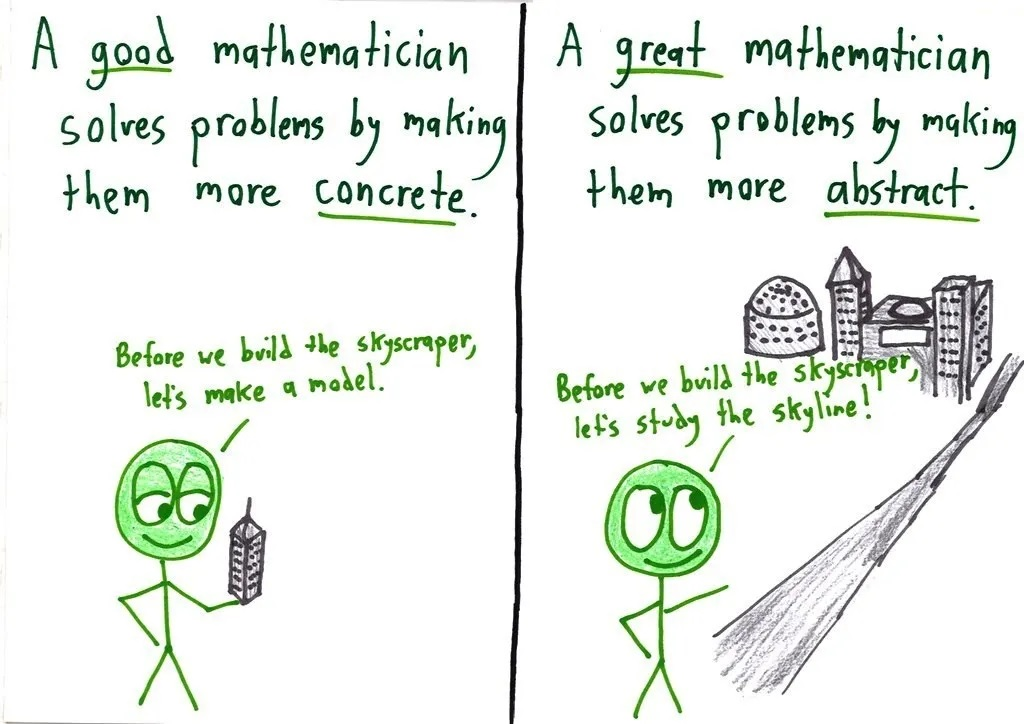
\includegraphics[width=0.65\textwidth]{GreatMath_5.jpg}
	\end{center}

 
%\thispagestyle{empty}
%\newpage\phantom{}


